\documentclass[11pt,oneside]{article}

\usepackage[a4paper,margin=25mm,headheight=15pt]{geometry}
\usepackage[T1]{fontenc}
\usepackage[utf8]{inputenc}
\IfFileExists{libertinus.sty}{\usepackage{libertinus}}{\usepackage{lmodern}}
\usepackage{microtype}
\usepackage{amsmath,amssymb,amsthm,mathtools,mathrsfs,bm}
% Canonical mathematical notation for active FabiusFunction LaTeX documents.
%
% This file is intentionally a plain TeX input rather than a LaTeX package.
% Every standalone document loads it by an explicit path relative to that
% document's directory; included fragments inherit the definitions from their
% root document.  Keep this file independent of document layout and metadata.
%
% Contract:
%   * one command has one mathematical meaning throughout the active corpus;
%   * names encode semantic roles rather than a document-local choice of letter;
%   * visually similar but differently normalized objects have different print;
%   * every command below is defined normatively in the notation catalogue.
%
% The active corpus excludes docs/archive/.  Historical sources may retain
% their original notation only inside an explicitly labelled quotation.

\makeatletter
\@ifundefined{mathbb}{%
  \PackageError{fabius-notation}{The amssymb package must be loaded first}%
    {Load amsmath and amssymb before inputting fabius-notation.tex.}%
}{}
\@ifundefined{operatorname}{%
  \PackageError{fabius-notation}{The amsmath package must be loaded first}%
    {Load amsmath before inputting fabius-notation.tex.}%
}{}
\makeatother

% Version stamp used by the catalogue and by static audits.
\newcommand{\FabiusNotationVersion}{2026-08-31}

% Number systems.  NaturalNumbers is explicitly the nonnegative convention.
\newcommand{\NaturalNumbers}{\mathbb{N}_{0}}
\newcommand{\PositiveIntegers}{\mathbb{N}_{>0}}
\newcommand{\IntegerNumbers}{\mathbb{Z}}
\newcommand{\RationalNumbers}{\mathbb{Q}}
\newcommand{\RealNumbers}{\mathbb{R}}
\newcommand{\ComplexNumbers}{\mathbb{C}}
\newcommand{\ExtendedRealNumbers}{\overline{\mathbb{R}}}

% The three principal Fabius--Rvachev functions.  Subscripts are deliberate:
% a bare F and a calligraphic F have several unrelated uses in the corpus.
\newcommand{\FabiusBounded}{F_{\mathrm{bd}}}
\newcommand{\FabiusGlobal}{F_{\mathrm{gl}}}
\newcommand{\FabiusQuantile}{Q_{F}}
\newcommand{\FabiusClampedQuantile}{Q_{F,\mathrm{cl}}}
\newcommand{\RvachevUp}{\operatorname{up}}

% Constants, elementary operators, and delimiters.
\newcommand{\EulerE}{\mathrm{e}}
\newcommand{\ImaginaryUnit}{\mathrm{i}}
\newcommand{\Differential}{\mathop{}\!\mathrm{d}}
\newcommand{\AbsoluteValue}[1]{\left\lvert #1\right\rvert}
\newcommand{\Norm}[1]{\left\lVert #1\right\rVert}
\newcommand{\Floor}[1]{\left\lfloor #1\right\rfloor}
\newcommand{\Ceiling}[1]{\left\lceil #1\right\rceil}
\newcommand{\FractionalPart}[1]{\left\{#1\right\}}
\newcommand{\PositivePart}[1]{\left(#1\right)_{+}}
\newcommand{\IndicatorOf}[1]{\mathbf{1}_{#1}}
\newcommand{\SetOf}[1]{\left\{#1\right\}}
\newcommand{\InnerProduct}[1]{\left\langle #1\right\rangle}
\newcommand{\CardinalityOf}[1]{\left\lvert #1\right\rvert}
\newcommand{\DefinitionEquals}{\mathrel{\coloneqq}}
\newcommand{\Sign}{\operatorname{sgn}}
\newcommand{\IdentityOperator}{\operatorname{id}}
\newcommand{\SpanOperator}{\operatorname{span}}
\newcommand{\TraceOperator}{\operatorname{tr}}
\newcommand{\RankOperator}{\operatorname{rank}}
\newcommand{\DiagonalOperator}{\operatorname{diag}}
\newcommand{\ResidueOperator}{\operatorname*{Res}}
\newcommand{\LeastCommonMultiple}{\operatorname{lcm}}
\newcommand{\OrderOperator}{\operatorname{ord}}
\newcommand{\PrincipalLogarithm}{\operatorname{Log}}
\newcommand{\FallingFactorial}[2]{\left(#1\right)^{\underline{#2}}}
\newcommand{\RisingFactorial}[2]{\left(#1\right)^{\overline{#2}}}

% Support, topology, convolution, and metric notation.
\newcommand{\SupportOperator}{\operatorname{supp}}
\newcommand{\SupportOf}[1]{\SupportOperator\!\left(#1\right)}
\newcommand{\TopologicalSupportOf}[1]{\operatorname{tsupp}\!\left(#1\right)}
\newcommand{\Convolution}{\mathbin{*}}
\newcommand{\MetricDistance}{\operatorname{dist}}
\newcommand{\TotalVariationDistance}{d_{\mathrm{TV}}}

% Probability.  Equality and convergence in law are not metric distance.
\newcommand{\Probability}{\mathbb{P}}
\newcommand{\Expectation}{\mathbb{E}}
\newcommand{\Variance}{\operatorname{Var}}
\newcommand{\Covariance}{\operatorname{Cov}}
\newcommand{\LawOperator}{\operatorname{Law}}
\newcommand{\LawOf}[1]{\LawOperator\!\left(#1\right)}
\newcommand{\EqualInLaw}{\mathrel{\overset{\mathrm{law}}{=}}}
\newcommand{\ConvergesInLaw}{\mathrel{\xrightarrow{\mathrm{law}}}}

% Fourier and integral transforms.  The printed labels expose normalization.
% FourierTwoPi uses exp(-2*pi*i*x*xi); FourierAngular uses exp(-i*x*omega).
\newcommand{\FourierTwoPi}[1]{\widehat{#1}_{\,2\pi}}
\newcommand{\FourierAngular}[1]{\widehat{#1}_{\,\mathrm{ang}}}
\newcommand{\LaplaceTransformSymbol}{\mathcal{L}}
\newcommand{\MellinTransformSymbol}{\mathcal{M}}
\newcommand{\LaplaceTransformOf}[1]{\LaplaceTransformSymbol\!\left[#1\right]}
\newcommand{\MellinTransformOf}[1]{\MellinTransformSymbol\!\left[#1\right]}
\newcommand{\MomentGeneratingFunction}[1]{M_{#1}}
\newcommand{\CharacteristicFunction}[1]{\varphi_{#1}}

% The two standard sinc functions must never share one symbol.
\newcommand{\SincRad}{\operatorname{sinc}_{\mathrm{rad}}}
\newcommand{\SincPi}{\operatorname{sinc}_{\pi}}

% Binary arithmetic and Thue--Morse notation.
\newcommand{\BinaryDigitSum}{\operatorname{wt}_{2}}
\newcommand{\ThueMorseSignSymbol}{\varepsilon}
\newcommand{\ThueMorseSign}[1]{\varepsilon_{#1}}
\newcommand{\PadicValuation}[1]{\nu_{#1}}
\newcommand{\TwoAdicValuation}{\nu_{2}}

% q-series notation.  Every base is an explicit argument.
\newcommand{\QPochhammer}[3]{\left(#1;#2\right)_{#3}}
\newcommand{\GaussianBinomial}[3]{%
  \genfrac{[}{]}{0pt}{}{#1}{#2}_{#3}%
}
\newcommand{\QInteger}[2]{\left[#1\right]_{#2}}

% Named special functions.
\newcommand{\Polylogarithm}{\operatorname{Li}}
\newcommand{\LambertW}{W}
\newcommand{\GammaFunction}{\Gamma}
\newcommand{\RiemannZeta}{\zeta}

% Asymptotics.  BigO and LittleO are operator tokens for existing formula
% grammar; prefer the At forms so that the limiting regime is printed.
\newcommand{\BigO}{\mathcal{O}}
\newcommand{\LittleO}{o}
\newcommand{\BigOAt}[2]{\mathcal{O}_{#2}\!\left(#1\right)}
\newcommand{\LittleOAt}[2]{o_{#2}\!\left(#1\right)}

\usepackage{booktabs,longtable,array,tabularx,multirow}
\usepackage{graphicx}
\usepackage{caption}
\usepackage{xcolor}
\usepackage{enumitem}
\usepackage{fancyhdr}
\usepackage{titlesec}
\usepackage{listings}
\usepackage{xurl}
\usepackage[hypertexnames=false]{hyperref}
\usepackage[nameinlink,noabbrev]{cleveref}
\usepackage{aliascnt}

\definecolor{linkblue}{RGB}{25,75,135}
\definecolor{deepgreen}{RGB}{28,103,76}
\definecolor{shadegray}{RGB}{246,247,249}
\definecolor{rulegray}{RGB}{195,201,208}
\hypersetup{
  colorlinks=true,
  linkcolor=linkblue,
  citecolor=deepgreen,
  urlcolor=linkblue,
  pdftitle={Legendre--Rvachev Biorthogonal Closure},
  pdfsubject={Finite shifted-up synthesis of Legendre polynomials, blockwise self-loop, dual kernels, rational spectral sum rules, and coefficient asymptotics},
  pdfkeywords={Rvachev up function, Legendre polynomials, Fabius function, Strang--Fix, infinite sinc product, spherical Bessel function, Bell polynomials, Bernoulli numbers, Thue--Morse, Lambert W}
}

\pagestyle{fancy}
\fancyhf{}
\fancyhead[L]{\small Legendre--Rvachev closure}
\fancyhead[R]{\small\nouppercase{\leftmark}}
\fancyfoot[C]{\thepage}
\renewcommand{\headrulewidth}{0.4pt}
\titleformat{\section}{\Large\bfseries}{\thesection}{0.7em}{}
\titleformat{\subsection}{\large\bfseries}{\thesubsection}{0.7em}{}
\titleformat{\subsubsection}{\normalsize\bfseries}{\thesubsubsection}{0.7em}{}
\setcounter{secnumdepth}{3}
\setcounter{tocdepth}{2}
\setlist[itemize]{leftmargin=2em,itemsep=0.25em,topsep=0.4em}
\setlist[enumerate]{leftmargin=2.3em,itemsep=0.25em,topsep=0.4em}
\setlength{\emergencystretch}{3em}
\allowdisplaybreaks[2]
\numberwithin{equation}{section}

\newtheorem{theorem}{Theorem}[section]
\newcommand{\newsharedtheorem}[2]{%
  \newaliascnt{#1}{theorem}%
  \newtheorem{#1}[#1]{#2}%
  \aliascntresetthe{#1}%
}
\newsharedtheorem{proposition}{Proposition}
\newsharedtheorem{lemma}{Lemma}
\newsharedtheorem{corollary}{Corollary}
\newsharedtheorem{identity}{Identity}
\newsharedtheorem{conjecture}{Conjecture}
\newsharedtheorem{problem}{Problem}
\newsharedtheorem{question}{Research question}
\theoremstyle{definition}
\newsharedtheorem{definition}{Definition}
\newsharedtheorem{algorithm}{Algorithm}
\newsharedtheorem{example}{Example}
\theoremstyle{remark}
\newsharedtheorem{remark}{Remark}
\newsharedtheorem{warning}{Warning}
\crefname{conjecture}{conjecture}{conjectures}
\Crefname{conjecture}{Conjecture}{Conjectures}
\crefname{problem}{problem}{problems}
\Crefname{problem}{Problem}{Problems}
\crefname{question}{research question}{research questions}
\Crefname{question}{Research question}{Research questions}
\crefname{identity}{identity}{identities}
\Crefname{identity}{Identity}{Identities}

\newcommand{\MM}{\mathsf M}
\newcommand{\Dscr}{\mathscr D_u}
\newcommand{\eps}{\varepsilon}
\newcommand{\tr}{\operatorname{tr}}
\newcommand{\repo}{\nolinkurl{Analysis/FabiusFunction/docs}}
\DeclareMathOperator{\ord}{ord}

\newenvironment{statusbox}[1]{%
  \par\smallskip\noindent\begin{center}\begin{minipage}{0.94\textwidth}%
  \hrule\vspace{0.55em}\noindent\textbf{#1}\par\smallskip
}{%
  \vspace{0.55em}\hrule\end{minipage}\end{center}\smallskip
}

\lstdefinestyle{pythonstyle}{
  language=Python,
  basicstyle=\ttfamily\footnotesize,
  backgroundcolor=\color{shadegray},
  frame=single,
  rulecolor=\color{rulegray},
  columns=fullflexible,
  keepspaces=true,
  showstringspaces=false,
  breaklines=true,
  xleftmargin=0.7em,
  xrightmargin=0.7em,
  aboveskip=0.8em,
  belowskip=0.8em
}

\title{\bfseries Legendre--Rvachev Biorthogonal Closure\\[0.45em]
\large Exact finite shifted-up synthesis, the blockwise self-loop,\\
dual translated moments, rational spectral sum rules, and log-square decay}
\author{Research report for Vladimir Reshetnikov's \texttt{ProveIt} project}
\date{29 August 2026}

\begin{document}
\maketitle

\begin{abstract}
Let $u=\RvachevUp$ be Rvachev's even $C^\infty$ probability density supported on
$[-1,1]$, and let $P_\ell$ be the Legendre polynomial normalized by
$P_\ell(1)=1$.  The repository already proves exact reproduction of every
polynomial by a finite local sum of shifted or shifted-and-dilated copies of
$u$, and it proves an absolutely and uniformly convergent Fourier--Legendre
series
\[
 u(x)=\sum_{n\ge0}u_nP_{2n}(x).
\]
This report specializes the first theorem to the Legendre basis, substitutes
it into the second theorem, and then develops the additional structure exposed
by that closure.

Put
\[
 \MM_u(z)=\int_{-1}^{1}\EulerE^{zx}u(x)\Differential x
 =\prod_{j\ge1}\frac{\sinh(z/2^j)}{z/2^j},
 \qquad
 \Dscr=\MM_u(D)^{-1},
 \qquad Q_\ell=\Dscr P_\ell.
\]
For any integer $M$ with $\TwoAdicValuation(M)\ge\ell$,
\[
 P_\ell(x)=\frac1M\sum_{|k|<2M}Q_\ell(k/M)u(x-k/M),
 \qquad -1\le x\le1.
\]
The deconvolved Legendre polynomial has the explicit Jacobi form
\[
 Q_\ell(x)=\sum_{r=0}^{\lfloor\ell/2\rfloor}
 \frac{\gamma_{2r}}{(2r)!}
 \frac{(\ell+2r)!}{2^{2r}\ell!}
 P_{\ell-2r}^{(2r,2r)}(x),
 \qquad
 \frac1{\MM_u(z)}=\sum_{r\ge0}\gamma_r\frac{z^r}{r!}.
\]
Choosing $M=4^n$ for $P_{2n}$ closes the requested loop:
\[
 u(x)=\sum_{n=0}^{\infty}\frac{u_n}{4^n}
 \sum_{|k|<2\cdot4^n}Q_{2n}(k/4^n)u(x-k/4^n).
\]
The outer series is absolutely and uniformly convergent only when every finite
inner sum is retained as a cancellation block; the adjacent repository report
proves that a flattened atom series is not absolute or unconditional.

The principal new structure here is a dual translated-moment kernel
\[
 \Lambda_m(c)=\frac{2m+1}{2}\int_{-1}^{1}u(x-c)P_m(x)\Differential x.
\]
It is compactly supported and smooth, satisfies
$\Lambda_{2n}(0)=u_n$, and has the spherical-Bessel representation
\[
 \Lambda_m(c)=(2m+1)(-\ImaginaryUnit)^m\int_{\RealNumbers}
 \widehat u(\xi)j_m(2\pi\xi)\EulerE^{2\pi\ImaginaryUnit\xi c}\Differential\xi.
\]
The finite Legendre synthesis and this dual analysis obey exact dyadic
biorthogonality:
\[
 \frac1M\sum_{|k|<2M}Q_\ell(k/M)\Lambda_m(k/M)=\delta_{m\ell}.
\]
Expanding every shifted atom back into local Legendre polynomials gives a
second closure.  It produces explicit rational coefficients
$T_{m\ell r}^{(M)}$ for which
\[
 \delta_{m\ell}=\sum_{r\ge0}u_rT_{m\ell r}^{(M)}.
\]
These are infinite rational spectral identities with exact parity blocks.
Endpoint flatness supplies a separate hierarchy of exact cancellation laws,
\[
 \sum_{r\ge\lceil s/2\rceil}u_r
 \frac{(2r+s)!}{2^ss!(2r-s)!}=0
 \qquad(s\ge0).
\]
Finally, the sharp real-axis sinc-product envelope from the repository, when
combined with the Bessel representation, yields the rigorous coefficient
bound
\[
 |u_n|\le C\frac{n^\sigma}{\log n}
 \exp\!\left(-\frac{(\log n)^2}{2\log2}\right)
\]
for an explicit finite $\sigma$.  Exact arithmetic through $n=80$ suggests
the new conjecture $\TwoAdicValuation(u_n)=-1$ for every $n$, while moments through
$\mu_{160}$ suggest
$\TwoAdicValuation(\mu_{2m}-1)=3+\TwoAdicValuation(m)$.  All numerical and symbolic experiments are
reproducible from the accompanying commented Python program.
\end{abstract}

\begin{statusbox}{Status and novelty discipline}
The Fourier product, probability model, moment and cumulant formulae, exact
polynomial synthesis, minimal $d+2$ endpoint dictionary, canonical
Fourier--Legendre expansion, reciprocal-MGF pole asymptotics, and the
non-flattening theorem are imported from the current \texttt{ProveIt} corpus.
The direct formula for $P_\ell$ is the requested basis specialization of the
existing polynomial theorem.  Claims described as ``new here'' are absent from
the canonical live exposition, the consolidated polynomial-synthesis volume,
and the directly adjacent Lagrange-loop report after a recursive inventory and
targeted full-text search at repository snapshot
\texttt{73c85cb0023615311fdc4a5ff4951767bddeff34}.  This is a corpus-relative
novelty statement, not an assertion of worldwide priority.  Every conjecture
is explicitly labeled; numerical evidence is never used in place of proof.
\end{statusbox}

\clearpage
\tableofcontents
\clearpage

\section{Corpus audit and orientation}
\label{sec:audit}

\subsection{The two transformations being composed}

The requested loop is a composition of two exact but analytically very
different maps.

First, the up-function generates polynomials locally.  For a polynomial $p$,
moment deconvolution produces another polynomial $\Dscr p$; samples of that
polynomial on a sufficiently oversampled dyadic lattice are coefficients of a
finite shifted-up representation of $p$ on a compact interval.  This is a
Strang--Fix phenomenon whose exact order is controlled by the integer-zero
multiplicities
\[
 \ord_{\xi=k}\widehat u(\xi)=1+\TwoAdicValuation(k)
 \qquad(k\in\IntegerNumbers\setminus\{0\}).
\]

Second, $u$ itself has a canonical orthogonal expansion in the even Legendre
basis.  Substituting the finite representation of each $P_{2n}$ gives a
self-representation of $u$.  The apparent circularity is not vacuous: the two
legs use different coordinate systems and different notions of convergence.
Moment deconvolution grows factorially with degree, whereas the outer Legendre
coefficients decay superalgebraically.  Their product is held together by
large finite cancellations.

\subsection{Sources used}

The recursive corpus inventory records the canonical exposition, archived
predecessors, the semi-formalized frontier collection, corrected source papers,
and live additions.  Mathematically duplicate snapshots were audited through
the repository's own provenance hashes rather than treated as independent
sources.  The report relies especially on:
\begin{itemize}
  \item the canonical volume \emph{The Fabius Function and Rvachev's
  Up-Function} \cite{ProveItPrimary};
  \item the consolidated volume \emph{Exact Polynomial Synthesis from
  Rvachev Up-Atoms} \cite{ProveItPoly};
  \item the immediately adjacent report \emph{Closing the
  Lagrange--Legendre--Rvachev Loop} \cite{ProveItLagrange};
  \item the historical and analytic sources of Fabius, Rvachev, and Arias de
  Reyna \cite{Fabius1966,Rvachev1971,Rvachev1972,Rvachev1990,Arias1982,Arias2018}.
\end{itemize}

\subsection{Imported and new results at a glance}

\begin{longtable}{@{}p{0.24\textwidth}p{0.70\textwidth}@{}}
\toprule
Status & Result \\
\midrule
\endfirsthead
\toprule Status & Result \\
\midrule
\endhead
Imported & Fourier sinc product, exact integer zero orders, probability law,
MGF, rational moments, Bernoulli cumulants, and rapid Fourier decay. \\
Imported & Exact polynomial synthesis on an interval, the minimal $d+2$ local
endpoint dictionary, and the dyadic $q$-integer/Thue--Morse annihilator. \\
Requested specialization & Explicit finite shifted-up representation of every
Legendre polynomial, including parity reduction and low-degree examples. \\
New here, corpus-relative & Jacobi-polynomial formula for the entire
Rvachev-deconvolved Legendre family $Q_\ell$. \\
Imported/requested composition & Exact blockwise
Legendre--up self-loop and fixed-scale partial-sum loop. \\
Imported from the adjacent report & Factorial asymptotic of $Q_{2n}(0)$ and
the theorem that the atom loop cannot be flattened absolutely or
unconditionally. \\
New here, corpus-relative & Dual translated Legendre kernel $\Lambda_m$,
its Bessel transform, support/parity/rationality, and exact dyadic
biorthogonality. \\
New here, corpus-relative & Reverse local-Legendre loop, clipped affine
connection coefficients, and the rational spectral identities
$\delta_{m\ell}=\sum_ru_rT_{m\ell r}^{(M)}$. \\
New here, corpus-relative & Endpoint-flatness coefficient sum rules and
finite boundary-jet identities tying the Legendre loop to dyadic derivative
cells and Thue--Morse signs. \\
New here, corpus-relative & A rigorous log-square upper bound on $|u_n|$
transferred from the sharp sinc-product Fourier envelope through spherical
Bessel functions. \\
New conjectures & Half-integrality of all $u_n$, a sharp moment congruence,
and dyadically modulated sharp asymptotics for the Legendre coefficients. \\
\bottomrule
\end{longtable}

\section{Foundations and notation}
\label{sec:foundations}

\subsection{The up density, Fourier transform, and probability model}

Let $u=\RvachevUp$ be the unique even nonnegative $C^\infty$ function supported on
$[-1,1]$, normalized by
\[
 \int_{-1}^{1}u(x)\Differential x=1,
 \qquad u(0)=1.
\]
We use the repository's Fourier convention
\[
 \widehat f(\xi)=\int_{\RealNumbers}f(x)\EulerE^{-2\pi\ImaginaryUnit\xi x}\Differential x.
\]
Then
\begin{equation}
 \widehat u(\xi)=\prod_{j=0}^{\infty}\SincPi(\xi/2^j),
 \qquad
 \SincPi(t)=\frac{\sin(\pi t)}{\pi t}.
 \label{eq:fourier-product}
\end{equation}
The zero at a nonzero integer $k$ has exact order $1+\TwoAdicValuation(k)$.
Equivalently, if $V_j$ are independent uniform random variables on $[-1,1]$,
then
\begin{equation}
 Z=\sum_{j\ge1}2^{-j}V_j
 \label{eq:probability-Z}
\end{equation}
has density $u$.  The distributional fixed point is
\begin{equation}
 Z\overset{d}=\frac{V+Z'}2,
 \label{eq:distribution-fixed-point}
\end{equation}
where $V$ is uniform on $[-1,1]$ and $Z'$ is an independent copy of $Z$.

\subsection{Moment generating function, moments, and cumulants}

The moment generating function is
\begin{equation}
 \MM_u(z)=\Expectation\EulerE^{zZ}
 =\int_{-1}^{1}\EulerE^{zx}u(x)\Differential x
 =\prod_{j\ge1}\frac{\sinh(z/2^j)}{z/2^j}.
 \label{eq:mgf}
\end{equation}
Write
\[
 \mu_r=\Expectation Z^r,
 \qquad
 \MM_u(z)=\sum_{r\ge0}\mu_r\frac{z^r}{r!}.
\]
All odd moments vanish.  From \eqref{eq:distribution-fixed-point}, for $m\ge1$,
\begin{equation}
 (4^m-1)\mu_{2m}
 =\sum_{r=1}^{m}\binom{2m}{2r}
   \frac{\mu_{2m-2r}}{2r+1}.
 \label{eq:moment-recurrence}
\end{equation}
Thus all moments are rational.  The first values are
\[
 \mu_0=1,
 \qquad \mu_2=\frac19,
 \qquad \mu_4=\frac{19}{675},
 \qquad \mu_6=\frac{583}{59535}.
\]
The cumulants are particularly simple:
\begin{equation}
 \log\MM_u(z)=\sum_{r\ge1}\kappa_r\frac{z^r}{r!},
 \qquad
 \kappa_{2r}=\frac{B_{2r}}{2r(1-4^{-r})},
 \qquad \kappa_{2r+1}=0,
 \label{eq:cumulants}
\end{equation}
where $B_{2r}$ are Bernoulli numbers.

\subsection{Moment deconvolution and its Bell--Bernoulli coefficients}

Define reciprocal coefficients by
\begin{equation}
 \frac1{\MM_u(z)}=\sum_{r=0}^{\infty}\gamma_r\frac{z^r}{r!}.
 \label{eq:gamma-def}
\end{equation}
Again, $\gamma_{2r+1}=0$.  On polynomials, the formal differential operator
\begin{equation}
 \Dscr:=\MM_u(D)^{-1}
 =\sum_{r\ge0}\gamma_r\frac{D^r}{r!}
 \label{eq:deconvolution}
\end{equation}
terminates exactly.  The reciprocal coefficients can be written with complete
exponential Bell polynomials:
\begin{equation}
 \gamma_n=Y_n(0,-\kappa_2,0,-\kappa_4,\ldots,-\kappa_n).
 \label{eq:gamma-bell}
\end{equation}
Consequently every exact coefficient below belongs to the algebra generated by
Bernoulli numbers and rational node coordinates.  The first even values are
\begin{equation}
 \gamma_0=1,
 \quad \gamma_2=-\frac19,
 \quad \gamma_4=\frac{31}{675},
 \quad \gamma_6=-\frac{2347}{59535},
 \quad \gamma_8=\frac{1904369}{32531625}.
 \label{eq:gamma-first}
\end{equation}

\subsection{Legendre and spherical-Bessel normalization}

The Legendre polynomials satisfy
\begin{equation}
 \int_{-1}^{1}P_m(x)P_n(x)\Differential x=\frac{2}{2n+1}\delta_{mn},
 \qquad \Norm{P_n}_{L^\infty[-1,1]}=1.
 \label{eq:legendre-orthogonality}
\end{equation}
Their Jacobi derivative formula is
\begin{equation}
 \frac{\Differential^s}{\Differential x^s}P_n(x)
 =2^{-s}\frac{(n+s)!}{n!}P_{n-s}^{(s,s)}(x),
 \qquad 0\le s\le n.
 \label{eq:legendre-jacobi-derivative}
\end{equation}
At the endpoint,
\begin{equation}
 P_n^{(s)}(1)=\frac{(n+s)!}{2^ss!(n-s)!}.
 \label{eq:legendre-endpoint-derivative}
\end{equation}
Finally, with $j_n$ denoting the spherical Bessel function,
\begin{equation}
 \int_{-1}^{1}P_n(x)\EulerE^{-\ImaginaryUnit tx}\Differential x=2(-\ImaginaryUnit)^n j_n(t).
 \label{eq:legendre-bessel}
\end{equation}
These normalizations fix all signs in the dual kernel developed later.

\section{Exact finite shifted-up synthesis of Legendre polynomials}
\label{sec:legendre-synthesis}

\subsection{The imported interval synthesis theorem}

The polynomial-synthesis volume proves the following physical-scale form.

\begin{theorem}[Exact unit-radius polynomial synthesis; imported]
\label{thm:general-synthesis}
Let $p$ be a polynomial of degree at most $d$, and let $M$ be a positive
integer satisfying $\TwoAdicValuation(M)\ge d$.  Then, for every $x\in[-1,1]$,
\begin{equation}
 p(x)=\frac1M\sum_{|k|<2M}(\Dscr p)(k/M)u(x-k/M).
 \label{eq:general-unit-radius}
\end{equation}
The sum is finite and contains $4M-1$ literal translates of the unscaled
function $u$.
\end{theorem}

\begin{proof}[Repository proof architecture]
Use spacing $h=M^{-1}$ and radius-to-spacing ratio $M$, so the physical atom
radius is one.  Poisson summation separates the zero-frequency polynomial
moment from aliases at nonzero integers.  The exact zero multiplicity
$1+\TwoAdicValuation(k)$ annihilates every alias derivative through degree $d$, while
$\MM_u(D)^{-1}$ reverses the zero-frequency convolution by the up law.  On
$[-1,1]$, the formal endpoint centers $k=\pm2M$ contribute only values at or
outside the support boundary and vanish, leaving \eqref{eq:general-unit-radius}.
\end{proof}

The minimal admissible power-of-two choice is $M=2^d$.  Larger $M$ with the
same or greater two-adic valuation gives the same reproduction order on a
finer lattice.

\subsection{Legendre specialization}

\begin{definition}[Rvachev-deconvolved Legendre family]
\label{def:Q}
For $\ell\ge0$, define
\begin{equation}
 Q_\ell(x):=\Dscr P_\ell(x).
 \label{eq:Q-def}
\end{equation}
\end{definition}

\begin{theorem}[Finite shifted-up representation of $P_\ell$]
\label{thm:legendre-synthesis}
Let $M$ be a positive integer with $\TwoAdicValuation(M)\ge\ell$.  Then
\begin{equation}
 \boxed{
 P_\ell(x)=\frac1M\sum_{|k|<2M}
 Q_\ell(k/M)u(x-k/M),
 \qquad -1\le x\le1.}
 \label{eq:legendre-synthesis}
\end{equation}
In particular, $M=2^\ell$ gives a canonical literal-shift representation with
$2^{\ell+2}-1$ displayed atoms.
\end{theorem}

\begin{proof}
Apply \cref{thm:general-synthesis} to $p=P_\ell$.  The definition
\eqref{eq:Q-def} is exactly the required deconvolution.
\end{proof}

This is the requested specialization of the arbitrary-polynomial result.  No
collocation system or numerical fitting is involved: the coefficient at the
center $k/M$ is an exact sample of one explicitly known degree-$\ell$
polynomial.

\subsection{A Jacobi-polynomial formula for $Q_\ell$}

The arbitrary-polynomial theorem alone does not exploit the special geometry
of the Legendre basis.  The derivative formula \eqref{eq:legendre-jacobi-derivative}
makes the specialization explicit.

\begin{theorem}[Jacobi form of the deconvolved Legendre polynomial; new here]
\label{thm:Q-jacobi}
For every $\ell\ge0$,
\begin{equation}
 \boxed{
 Q_\ell(x)=
 \sum_{r=0}^{\Floor{\ell/2}}
 \frac{\gamma_{2r}}{(2r)!}
 \frac{(\ell+2r)!}{2^{2r}\ell!}
 P_{\ell-2r}^{(2r,2r)}(x).}
 \label{eq:Q-jacobi}
\end{equation}
Consequently $Q_\ell\in\RationalNumbers[x]$ and
\begin{equation}
 Q_\ell(-x)=(-1)^\ell Q_\ell(x).
 \label{eq:Q-parity}
\end{equation}
\end{theorem}

\begin{proof}
Insert \eqref{eq:legendre-jacobi-derivative} with $s=2r$ into the terminating
operator \eqref{eq:deconvolution}.  Odd reciprocal coefficients vanish.  The
Jacobi polynomial $P_{\ell-2r}^{(2r,2r)}$ has parity
$(-1)^{\ell-2r}=(-1)^\ell$, proving \eqref{eq:Q-parity}.  Rationality follows
from rationality of $\gamma_{2r}$ and the standard rational coefficients of
Jacobi polynomials with integral parameters.
\end{proof}

\begin{remark}[Bell--Bernoulli content]
Combining \eqref{eq:Q-jacobi}, \eqref{eq:gamma-bell}, and
\eqref{eq:cumulants} expresses every shifted-up coefficient in
\eqref{eq:legendre-synthesis} as a finite combination of Jacobi values,
complete Bell polynomials, and Bernoulli numbers.  Thus the Bell--Bernoulli
structure is the exact inverse-smoothing mechanism, not merely a change of
notation.
\end{remark}

\subsection{Parity-reduced atom blocks}

The symmetry of $Q_\ell$ and $u$ halves the independent coefficient data.

\begin{corollary}[Even and odd paired forms]
\label{cor:paired-synthesis}
If $\ell$ is even, then
\begin{equation}
 P_\ell(x)=\frac{Q_\ell(0)}M u(x)
 +\frac1M\sum_{k=1}^{2M-1}Q_\ell(k/M)
 \bigl[u(x-k/M)+u(x+k/M)\bigr].
 \label{eq:even-paired}
\end{equation}
If $\ell$ is odd, then
\begin{equation}
 P_\ell(x)=\frac1M\sum_{k=1}^{2M-1}Q_\ell(k/M)
 \bigl[u(x-k/M)-u(x+k/M)\bigr].
 \label{eq:odd-paired}
\end{equation}
\end{corollary}

\begin{proof}
Pair the terms indexed by $k$ and $-k$ in
\eqref{eq:legendre-synthesis} and use \eqref{eq:Q-parity}.
\end{proof}

\subsection{Low-degree polynomials and exact examples}

The first deconvolved Legendre polynomials are:
% Generated by experiments.py
\begin{align*}
Q_{0}(x)&=1,\\
Q_{1}(x)&=x,\\
Q_{2}(x)&=\frac{3}{2}x^{2} - \frac{2}{3},\\
Q_{3}(x)&=\frac{5}{2}x^{3} - \frac{7}{3}x,\\
Q_{4}(x)&=\frac{35}{8}x^{4} - \frac{20}{3}x^{2} + \frac{134}{135},\\
Q_{5}(x)&=\frac{63}{8}x^{5} - \frac{35}{2}x^{3} + \frac{33}{5}x,\\
Q_{6}(x)&=\frac{231}{16}x^{6} - \frac{175}{4}x^{4} + \frac{889}{30}x^{2} - \frac{1426}{567}.
\end{align*}


For $\ell=0$, $M=1$, \cref{thm:legendre-synthesis} is the partition of unity
\begin{equation}
 1=u(x+1)+u(x)+u(x-1),
 \qquad -1\le x\le1.
 \label{eq:P0-example}
\end{equation}
For $\ell=1$, $M=2$,
\begin{equation}
 x=\frac14\sum_{k=-3}^{3}k\,u(x-k/2).
 \label{eq:P1-example}
\end{equation}
For $\ell=2$, $M=4$,
\begin{equation}
 P_2(x)=\sum_{k=-7}^{7}\frac{9k^2-64}{384}\,u(x-k/4).
 \label{eq:P2-example}
\end{equation}
These identities hold on the whole closed interval, including endpoints.

\subsection{The compressed $\ell+2$-atom representation}

Literal unit-radius shifts make the formula transparent but require
exponentially many displayed centers.  The repository's local dimension
theorem compresses any degree-$\ell$ polynomial to $\ell+2$ atoms at a large
common dilation.

Put $M=2^\ell$, $t=(x+1)/2$, and
\begin{equation}
 R_\ell(t)=P_\ell(2t-1),
 \qquad
 \widetilde Q_\ell(t)=\MM_u(MD_t)^{-1}R_\ell(t).
 \label{eq:compressed-Q}
\end{equation}
Let
\begin{equation}
 A_\ell(z)=\prod_{j=1}^{\ell}[2^j]_z,
 \qquad [N]_z=1+z+\cdots+z^{N-1}.
 \label{eq:q-annihilator}
\end{equation}
Its degree is $2M-\ell-2$.  The complete local alias nullspace is generated by
this $q$-integer product; after subtracting the unique null sequence matching
the left coefficients, only the centers
\begin{equation}
 M-\ell-1\le k\le M
 \label{eq:compressed-centers}
\end{equation}
remain.

\begin{theorem}[Compressed Legendre synthesis; imported specialization]
\label{thm:compressed-legendre}
There are unique rational coefficients $b_{\ell,k}$, with $k$ in
\eqref{eq:compressed-centers}, such that
\begin{equation}
 \boxed{
 P_\ell(x)=\frac1M\sum_{k=M-\ell-1}^{M}b_{\ell,k}
 u\!\left(\frac{x+1-2k}{2M}\right),
 \qquad -1\le x\le1.}
 \label{eq:compressed-legendre}
\end{equation}
Thus only $\ell+2$ shifted-and-dilated up-atoms are needed.
\end{theorem}

\begin{algorithm}[Exact coefficient compression]
\label{alg:compression}
Write $A_\ell(z)=\sum_{r=0}^{R}a_rz^r$ with $a_R=1$.  On the full active
integer interval $-M+1\le k\le M$, initialize a null sequence by matching
$n_k=\widetilde Q_\ell(k)$ on the first $R$ positions and extend it by
\begin{equation}
 n_{s+R}=-\sum_{r=0}^{R-1}a_rn_{s+r}.
 \label{eq:null-recurrence}
\end{equation}
Then
\begin{equation}
 b_{\ell,k}=\widetilde Q_\ell(k)-n_k,
 \qquad M-\ell-1\le k\le M.
 \label{eq:compressed-coeffs}
\end{equation}
All operations are exact in $\RationalNumbers$.
\end{algorithm}

The price of linear atom count is a dilation of order $2^\ell$ and substantial
coefficient cancellation.  The literal and compressed formulas therefore
occupy opposite ends of a scale--cardinality--conditioning tradeoff.

\section{The canonical Fourier--Legendre expansion and the requested loop}
\label{sec:canonical-loop}

\subsection{Exact Legendre coefficients}

The canonical repository expansion is
\begin{equation}
 u(x)=\sum_{n=0}^{\infty}u_nP_{2n}(x),
 \qquad
 u_n=\frac{4n+1}{2}\int_{-1}^{1}u(x)P_{2n}(x)\Differential x.
 \label{eq:canonical-expansion}
\end{equation}
It converges absolutely and uniformly on $[-1,1]$.  Expanding $P_{2n}$ in
monomials gives the exact moment formula
\begin{equation}
 \boxed{
 u_n=\frac{4n+1}{2^{2n+1}}
 \sum_{s=0}^{n}(-1)^{n-s}
 \frac{(2n+2s)!}{(n-s)!(n+s)!(2s)!}\,\mu_{2s}.}
 \label{eq:un-moments}
\end{equation}
Thus $u_n\in\RationalNumbers$.

\begin{center}
\small
% Generated by experiments.py
\begin{tabular}{@{}rllr@{}}
\toprule
$n$ & exact $u_n$ & decimal value & $v_2(u_n)$ \\
\midrule
0 & $\frac{1}{2}$ & $0.5$ & $-1$ \\
1 & $-\frac{5}{6}$ & $-0.8333333333$ & $-1$ \\
2 & $\frac{11}{30}$ & $0.3666666667$ & $-1$ \\
3 & $\frac{143}{5670}$ & $0.02522045855$ & $-1$ \\
4 & $-\frac{7291}{85050}$ & $-0.0857260435$ & $-1$ \\
5 & $\frac{99137}{2485890}$ & $0.03987988205$ & $-1$ \\
6 & $-\frac{5726162257}{213774110550}$ & $-0.02678604178$ & $-1$ \\
7 & $\frac{27288832157947}{1167420417713550}$ & $0.02337532541$ & $-1$ \\
8 & $-\frac{144048691053129139}{11591954102251136250}$ & $-0.01242660985$ & $-1$ \\
9 & $\frac{245262858648906702103531}{100278737599471847129463750}$ & $0.002445811191$ & $-1$ \\
10 & $\frac{190920333865973179103798951}{82729958519564273881807593750}$ & $0.002307753289$ & $-1$ \\
11 & $-\frac{45956358119729097218525273579033}{23132967547232266175685815725893750}$ & $-0.001986617498$ & $-1$ \\
\bottomrule
\end{tabular}

\end{center}

\subsection{Termwise finite closure}

For $P_{2n}$, take the minimal power-of-two ratio
\begin{equation}
 M_n=2^{2n}=4^n.
 \label{eq:Mn}
\end{equation}
Then \cref{thm:legendre-synthesis} gives
\begin{equation}
 P_{2n}(x)=\frac1{4^n}
 \sum_{|k|<2\cdot4^n}Q_{2n}(k/4^n)u(x-k/4^n).
 \label{eq:P2n-atomization}
\end{equation}

\begin{theorem}[Blockwise Legendre--Rvachev self-loop]
\label{thm:block-loop}
For every $x\in[-1,1]$,
\begin{equation}
 \boxed{
 u(x)=\sum_{n=0}^{\infty}\frac{u_n}{4^n}
 \sum_{|k|<2\cdot4^n}Q_{2n}(k/4^n)u(x-k/4^n).}
 \label{eq:block-loop}
\end{equation}
The outer series is absolutely and uniformly convergent when each finite inner
sum is retained as one block.
\end{theorem}

\begin{proof}
Substitute \eqref{eq:P2n-atomization} into
\eqref{eq:canonical-expansion}.  The $n$th finite inner sum is exactly
$P_{2n}(x)$, so its full block is $u_nP_{2n}(x)$.  Since
$\Norm{P_{2n}}_\infty=1$ and the canonical expansion is absolutely uniformly
convergent,
\[
 \sum_{n\ge0}\Norm{u_nP_{2n}}_\infty=\sum_{n\ge0}|u_n|<\infty.
\]
\end{proof}

Equation \eqref{eq:block-loop} is the requested closed loop.  It is an exact
series of finite self-reconstruction operators; it is not a tautological
pointwise insertion because the atom coefficients are explicit rational
samples of the deconvolved Legendre polynomials.

\subsection{One lattice for an entire partial sum}

Define
\begin{equation}
 S_N(x)=\sum_{n=0}^{N}u_nP_{2n}(x),
 \qquad
 C_N(x)=\Dscr S_N(x)=\sum_{n=0}^{N}u_nQ_{2n}(x).
 \label{eq:SN-CN}
\end{equation}
Since $\deg S_N=2N$, the single ratio $M=4^N$ reproduces the whole partial sum.

\begin{corollary}[Fixed-scale finite self-approximants]
\label{cor:fixed-scale}
For $x\in[-1,1]$,
\begin{equation}
 \boxed{
 S_N(x)=\frac1{4^N}
 \sum_{|k|<2\cdot4^N}C_N(k/4^N)u(x-k/4^N).}
 \label{eq:fixed-scale-loop}
\end{equation}
Every coefficient is rational, and the right side converges uniformly to $u$
as $N\to\infty$.
\end{corollary}

Applying the compressed dictionary to $S_N$ reduces the atom count to
$2N+2$, again at the price of dilation by $4^N$ and much larger cancellation.

\subsection{Why the loop must remain blockwise}

The adjacent Lagrange-loop report analyzes the repeated central copy $u(x)$ in
\eqref{eq:block-loop}.  With
\begin{equation}
 C_*=\MM_u(\pi\ImaginaryUnit)
 =\prod_{j\ge1}\frac{\sin(\pi/2^j)}{\pi/2^j},
 \label{eq:Cstar}
\end{equation}
it proves
\begin{equation}
 Q_{2n}(0)=
 \frac{2(-1)^n}{C_*}\frac{(4n)!}{(2n)!(4\pi)^{2n}}
 \left(1+\frac{2\pi^2}{4n-1}+\BigO(n^{-2})\right).
 \label{eq:Q0-asymptotic}
\end{equation}
In particular,
\begin{equation}
 |Q_{2n}(0)|^{1/(2n)}\sim\frac{2n}{\pi\EulerE}.
 \label{eq:Q0-root}
\end{equation}
The same report proves that
\begin{equation}
 \beta_n:=\frac{u_nQ_{2n}(0)}{4^n}
 \label{eq:central-beta}
\end{equation}
is unbounded in absolute value.  Otherwise $u_n$ would decay
supergeometrically, forcing an analytic continuation of $u$ across its flat
support endpoints, an impossibility for a nonzero compactly supported
$C^\infty$ function.  Therefore the double atom series cannot be flattened
into an absolutely or unconditionally convergent scalar series.  Increasingly
large signed coefficients cancel inside the $n$th block to leave the small
function $u_nP_{2n}$.

\begin{warning}[Legal and illegal rearrangements]
Finite regrouping inside one block is always legitimate, and the outer block
series may be rearranged absolutely.  Grouping all copies with the same center
across infinitely many degrees is not justified in general; the central
coefficient sequence alone is unbounded.
\end{warning}

\section{A dual translated Legendre kernel}
\label{sec:dual-kernel}

The finite synthesis coefficients $Q_\ell(k/M)$ analyze a polynomial before
placing up-atoms.  To close the transform in the opposite direction, we need
the Legendre coefficients of a shifted up-atom.

\begin{definition}[Translated Legendre analysis kernel]
\label{def:Lambda}
For $m\ge0$ and $c\in\RealNumbers$, define
\begin{equation}
 \boxed{
 \Lambda_m(c):=\frac{2m+1}{2}
 \int_{-1}^{1}u(x-c)P_m(x)\Differential x.}
 \label{eq:Lambda-def}
\end{equation}
\end{definition}

\subsection{Elementary properties}

\begin{proposition}[Support, smoothness, probability form, and parity; new here]
\label{prop:Lambda-basic}
For every $m\ge0$:
\begin{enumerate}
  \item $\Lambda_m\in C_c^\infty(\RealNumbers)$ and
        $\SupportOperator\Lambda_m\subseteq[-2,2]$;
  \item if $Z$ has density $u$, then
  \begin{equation}
   \Lambda_m(c)=\frac{2m+1}{2}\,
   \Expectation\!\left[P_m(c+Z)\mathbf1_{\{|c+Z|\le1\}}\right];
   \label{eq:Lambda-probability}
  \end{equation}
  \item
  \begin{equation}
   \Lambda_m(-c)=(-1)^m\Lambda_m(c);
   \label{eq:Lambda-parity}
  \end{equation}
  \item at the origin,
  \begin{equation}
   \Lambda_{2n}(0)=u_n,
   \qquad \Lambda_{2n+1}(0)=0.
   \label{eq:Lambda-origin}
  \end{equation}
\end{enumerate}
\end{proposition}

\begin{proof}
Let $\chi_m(x)=P_m(x)\mathbf1_{[-1,1]}(x)$.  Since $u$ is even,
\[
 \Lambda_m(c)=\frac{2m+1}{2}(u*\chi_m)(c).
\]
Convolution of a compactly supported $C^\infty$ function with a compactly
supported integrable function is $C^\infty$; supports add, giving $[-2,2]$.
Changing variables $x=c+z$ gives \eqref{eq:Lambda-probability}.  Reflection
$x\mapsto-x$, together with evenness of $u$ and parity of $P_m$, proves
\eqref{eq:Lambda-parity}.  Finally, \eqref{eq:Lambda-origin} is the definition
of the canonical Legendre coefficient, with odd terms zero by symmetry.
\end{proof}

Thus the original coefficients $u_n$ are merely the central samples of a much
larger family of translated Legendre moments.

\subsection{Spherical-Bessel transform}

\begin{theorem}[Fourier--Bessel representation of $\Lambda_m$; new here]
\label{thm:Lambda-bessel}
For all $m\ge0$ and $c\in\RealNumbers$,
\begin{equation}
 \boxed{
 \Lambda_m(c)=(2m+1)(-\ImaginaryUnit)^m
 \int_{\RealNumbers}\widehat u(\xi)j_m(2\pi\xi)
 \EulerE^{2\pi\ImaginaryUnit\xi c}\Differential\xi.}
 \label{eq:Lambda-bessel}
\end{equation}
In particular,
\begin{equation}
 \boxed{
 u_n=(4n+1)(-1)^n
 \int_{\RealNumbers}\widehat u(\xi)j_{2n}(2\pi\xi)\Differential\xi.}
 \label{eq:un-bessel}
\end{equation}
\end{theorem}

\begin{proof}
The Fourier transform of $\chi_m$ is, by
\eqref{eq:legendre-bessel},
\[
 \widehat\chi_m(\xi)=2(-\ImaginaryUnit)^m j_m(2\pi\xi).
\]
Since $\Lambda_m=(2m+1)(u*\chi_m)/2$, Fourier inversion gives
\eqref{eq:Lambda-bessel}.  Set $c=0$ and $m=2n$ to obtain
\eqref{eq:un-bessel}.
\end{proof}

Equation \eqref{eq:un-bessel} is the analytic bridge between the repository's
sharp sinc-product Fourier envelope and the Legendre coefficients.  It also
suggests that dyadic Fourier-lobe structure should survive as a modulation in
$u_n$.

\subsection{Exact rationality at dyadic shifts}

\begin{proposition}[Dyadic rationality of the dual samples; new here]
\label{prop:Lambda-rational}
If $c$ is dyadic rational, then $\Lambda_m(c)\in\RationalNumbers$ for every $m$.
\end{proposition}

\begin{proof}
After $x=c+y$,
\[
 \Lambda_m(c)=\frac{2m+1}{2}
 \int_{[-1,1]\cap[-1-c,1-c]}u(y)P_m(y+c)\Differential y.
\]
The endpoints are dyadic.  Expand $P_m(y+c)$ into powers of $y$.  The
repository's exact dyadic primitive calculus expresses every truncated moment
$\int_a^b y^r u(y)\Differential y$ at dyadic endpoints in rational Fabius/up values and
rational polynomial factors.  Hence the displayed finite linear combination
is rational.
\end{proof}

The accompanying code does not need to evaluate $u$ to compute the later
connection coefficients; it integrates the corresponding clipped Legendre
polynomials exactly in $\RationalNumbers$.

\section{Exact dyadic spectral biorthogonality}
\label{sec:biorthogonality}

\subsection{The scalar identity}

\begin{theorem}[Legendre--up dyadic biorthogonality; new here]
\label{thm:biorthogonality}
Let $d\ge0$, $M=2^d$, $0\le\ell\le d$, and $m\ge0$.  Then
\begin{equation}
 \boxed{
 \frac1M\sum_{|k|<2M}Q_\ell(k/M)\Lambda_m(k/M)
 =\delta_{m\ell}.}
 \label{eq:biorthogonality}
\end{equation}
More generally, the same identity holds for any positive integer $M$ with
$\TwoAdicValuation(M)\ge\ell$.
\end{theorem}

\begin{proof}
Use the admissible common-scale representation
\[
 P_\ell(x)=\frac1M\sum_{|k|<2M}Q_\ell(k/M)u(x-k/M).
\]
Multiply by $(2m+1)P_m(x)/2$ and integrate over $[-1,1]$.  Orthogonality gives
$\delta_{m\ell}$ on the left, while the integral of the shifted atom is exactly
$\Lambda_m(k/M)$ by \cref{def:Lambda}.
\end{proof}

For each fixed $\ell$, \eqref{eq:biorthogonality} is an infinite family of
finite identities indexed by $m$.  The cases $m>\ell$ say that the finite
coefficient row annihilates all higher translated Legendre moments exactly.

\subsection{Parity blocks}

From \eqref{eq:Q-parity} and \eqref{eq:Lambda-parity}, the summand in
\eqref{eq:biorthogonality} changes by $(-1)^{m+\ell}$ under $k\mapsto-k$.
Therefore opposite parities cancel term by term.  For equal parity,
\begin{equation}
 \delta_{m\ell}
 =\frac{Q_\ell(0)\Lambda_m(0)}M
 +\frac2M\sum_{k=1}^{2M-1}
 Q_\ell(k/M)\Lambda_m(k/M),
 \label{eq:biorthogonality-paired}
\end{equation}
where the central term vanishes automatically in the odd--odd block.

\subsection{Finite analysis and synthesis matrices}

Let
\[
 \mathcal K_M=\{k\in\IntegerNumbers:|k|<2M\}.
\]
For $0\le m,\ell\le d$, define
\begin{equation}
 A^{(d)}_{k\ell}=\frac1M Q_\ell(k/M),
 \qquad
 L^{(d)}_{mk}=\Lambda_m(k/M).
 \label{eq:AL-matrices}
\end{equation}
Then $A^{(d)}$ is a $(4M-1)\times(d+1)$ synthesis matrix and $L^{(d)}$ is a
$(d+1)\times(4M-1)$ analysis matrix.

\begin{corollary}[Exact spectral right inverse and oblique projector]
\label{cor:spectral-projector}
The matrices in \eqref{eq:AL-matrices} satisfy
\begin{equation}
 \boxed{L^{(d)}A^{(d)}=I_{d+1}.}
 \label{eq:LA-I}
\end{equation}
Consequently
\begin{equation}
 \Pi^{(d)}:=A^{(d)}L^{(d)},
 \qquad
 (\Pi^{(d)})^2=\Pi^{(d)},
 \qquad
 \RankOperator\Pi^{(d)}=\tr\Pi^{(d)}=d+1.
 \label{eq:spectral-projector}
\end{equation}
The even and odd Legendre modes form independent parity blocks.
\end{corollary}

This is the spectral counterpart of the nodal right inverse in the adjacent
Lagrange report.  There, analysis consists of point evaluation at interpolation
nodes.  Here, analysis consists of exact Legendre moments of shifted atoms.

\begin{corollary}[Trace and Cauchy--Binet identities]
\label{cor:trace-cauchy-binet}
One has
\begin{equation}
 \frac1M\sum_{k\in\mathcal K_M}
 \sum_{\ell=0}^{d}Q_\ell(k/M)\Lambda_\ell(k/M)=d+1,
 \label{eq:trace-identity}
\end{equation}
and
\begin{equation}
 1=\sum_{\substack{S\subset\mathcal K_M\\|S|=d+1}}
 \det L^{(d)}_{:,S}\,\det A^{(d)}_{S,:}.
 \label{eq:spectral-cauchy-binet}
\end{equation}
\end{corollary}

\begin{proof}
Take the trace and determinant, respectively, of
$L^{(d)}A^{(d)}=I$; the determinant expansion is Cauchy--Binet.
\end{proof}

\section{The reverse local-Legendre loop}
\label{sec:reverse-loop}

The requested self-loop substitutes an up-atom representation into a Legendre
series.  We can also expand each shifted atom back into Legendre polynomials in
its own local coordinate.  The support clipping is essential.

\subsection{Shifted local expansions}

For $c\in[-2,2]$, define the overlap interval
\begin{equation}
 I(c)=[-1,1]\cap[c-1,c+1].
 \label{eq:overlap-interval}
\end{equation}
The canonical series implies, uniformly for real $x$,
\begin{equation}
 u(x-c)=\mathbf1_{I(c)}(x)
 \sum_{r=0}^{\infty}u_rP_{2r}(x-c).
 \label{eq:shifted-local-expansion}
\end{equation}
Indeed, inside the support this is the canonical expansion in the coordinate
$x-c$, and outside both sides vanish.  Absolute uniform convergence survives
multiplication by the indicator because $\sum_r|u_r|<\infty$ and
$|P_{2r}|\le1$ on $[-1,1]$.

For admissible $M$, define the piecewise-polynomial block
\begin{equation}
 H_{\ell r}^{(M)}(x)=\frac1M\sum_{|k|<2M}
 Q_\ell(k/M)\mathbf1_{I(k/M)}(x)P_{2r}(x-k/M).
 \label{eq:H-def}
\end{equation}
Its knots belong to the dyadic grid generated by the endpoints
$k/M\pm1$.

\begin{theorem}[Reverse local-Legendre closure; new here]
\label{thm:reverse-loop}
If $\TwoAdicValuation(M)\ge\ell$, then on $[-1,1]$,
\begin{equation}
 \boxed{
 P_\ell(x)=\sum_{r=0}^{\infty}u_rH_{\ell r}^{(M)}(x).}
 \label{eq:reverse-loop}
\end{equation}
The series converges absolutely and uniformly.
\end{theorem}

\begin{proof}
Insert \eqref{eq:shifted-local-expansion} into the finite synthesis formula
\eqref{eq:legendre-synthesis}.  Since the outer atom sum is finite and each
local Legendre series is absolutely uniform, interchange of the two sums is
legitimate.  The coefficient of $u_r$ is exactly \eqref{eq:H-def}.
\end{proof}

Although each $H_{\ell r}^{(M)}$ is only piecewise polynomial, the infinite
weighted sum is the globally smooth polynomial $P_\ell$.  All jumps of all
piecewise derivatives cancel.  \Cref{sec:flatness} identifies the endpoint
sum rules responsible for this phenomenon.

\subsection{Clipped affine Legendre connection coefficients}

Project the local expansion against a global Legendre mode.  Define
\begin{equation}
 \boxed{
 C_{m,r}(c)=\frac{2m+1}{2}
 \int_{I(c)}P_m(x)P_{2r}(x-c)\Differential x.}
 \label{eq:Cmr-def}
\end{equation}
For rational $c$, this is rational because it is the integral of a polynomial
over an interval with rational endpoints.  Reflection gives
\begin{equation}
 C_{m,r}(-c)=(-1)^mC_{m,r}(c).
 \label{eq:Cmr-parity}
\end{equation}

\begin{proposition}[Local connection expansion of the dual kernel; new here]
\label{prop:Lambda-connection}
For every $m\ge0$ and $c\in[-2,2]$,
\begin{equation}
 \boxed{
 \Lambda_m(c)=\sum_{r=0}^{\infty}u_rC_{m,r}(c).}
 \label{eq:Lambda-C-expansion}
\end{equation}
The series converges absolutely and uniformly in $c$.
\end{proposition}

\begin{proof}
Insert \eqref{eq:shifted-local-expansion} into
\eqref{eq:Lambda-def} and integrate termwise.  Uniformity follows from
$|P_m|\le1$, $|P_{2r}|\le1$ on their respective intervals, interval length at
most two, and $\sum_r|u_r|<\infty$.
\end{proof}

\subsection{Arithmetic spectral closure}

For $\TwoAdicValuation(M)\ge\ell$, define
\begin{equation}
 \boxed{
 T_{m\ell r}^{(M)}=
 \frac1M\sum_{|k|<2M}Q_\ell(k/M)C_{m,r}(k/M).}
 \label{eq:T-def}
\end{equation}
Every $T_{m\ell r}^{(M)}$ is rational.

\begin{theorem}[Infinite rational spectral identities; new here]
\label{thm:rational-spectral-closure}
For every $m,\ell\ge0$ and every admissible $M$ with
$\TwoAdicValuation(M)\ge\ell$,
\begin{equation}
 \boxed{
 \delta_{m\ell}=\sum_{r=0}^{\infty}u_rT_{m\ell r}^{(M)}.}
 \label{eq:rational-spectral-closure}
\end{equation}
Moreover,
\begin{equation}
 m+\ell\ \text{odd}
 \quad\Longrightarrow\quad
 T_{m\ell r}^{(M)}=0
 \quad\text{for every }r.
 \label{eq:T-parity-zero}
\end{equation}
\end{theorem}

\begin{proof}
Substitute \eqref{eq:Lambda-C-expansion} into the finite biorthogonality
identity \eqref{eq:biorthogonality}.  The finite sum over $k$ may be
interchanged with the absolutely convergent series over $r$, giving
\eqref{eq:rational-spectral-closure}.  Rationality follows from rationality of
$Q_\ell(k/M)$ and $C_{m,r}(k/M)$.  Finally,
$Q_\ell(-c)C_{m,r}(-c)=(-1)^{m+\ell}Q_\ell(c)C_{m,r}(c)$;
opposite parity therefore cancels in symmetric pairs, while the central term
vanishes when appropriate.
\end{proof}

This theorem converts an analytic orthogonality relation into infinitely many
identities involving only rational numbers.  All transcendental content has
been isolated in the universal coefficient sequence $(u_r)$.

\subsection{Exact examples}

For $(\ell,m)=(1,1)$ and $M=2$, the first connection constants are
\begin{equation}
 \left(T_{11r}^{(2)}\right)_{r\ge0}=
 \left(
 \frac{15}{8},
 -\frac{15}{128},
 -\frac{85}{1024},
 -\frac{267}{32768},
 \frac{11949}{262144},
 -\frac{128339}{4194304},
 \ldots\right),
 \label{eq:T11-values}
\end{equation}
and \eqref{eq:rational-spectral-closure} says
\begin{equation}
 1=\sum_{r\ge0}u_rT_{11r}^{(2)}.
 \label{eq:T11-identity}
\end{equation}
For $(\ell,m)=(2,2)$, $M=4$,
\begin{equation}
 \left(T_{22r}^{(4)}\right)_{r\ge0}=
 \left(
 \frac{945}{512},
 -\frac{29737}{196608},
 -\frac{291095}{2097152},
 -\frac{28532595}{268435456},
 -\frac{400224525}{8589934592},
 \ldots\right),
 \label{eq:T22-values}
\end{equation}
again summing to one after weighting by $u_r$.  In contrast,
\begin{equation}
 \left(T_{20r}^{(4)}\right)_{r\ge0}=
 \left(
 \frac{61}{96},
 \frac{189}{512},
 -\frac{945}{32768},
 -\frac{24003}{1048576},
 -\frac{1504629}{134217728},
 \ldots\right)
 \label{eq:T20-values}
\end{equation}
has weighted sum zero.  Every $T_{21r}^{(4)}$ is exactly zero by parity.

\begin{figure}[htbp]
\centering
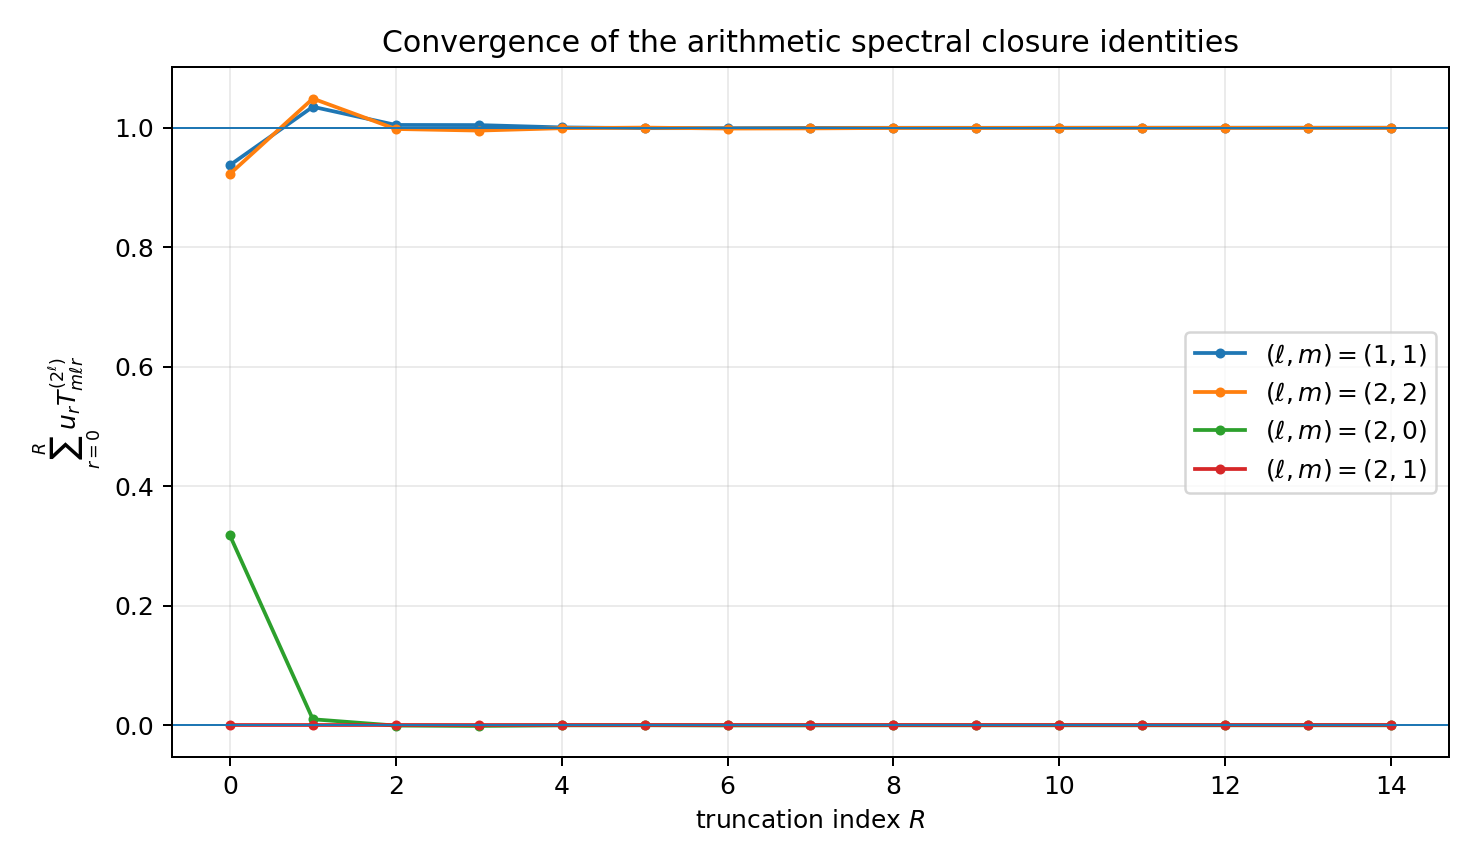
\includegraphics[width=0.94\textwidth]{spectral_sum_convergence.png}
\caption{Partial sums of four exact rational spectral identities.  Decimal
plotting is used only for visualization; the coefficients and all partial sums
in the accompanying CSV file are computed in exact rational arithmetic.}
\label{fig:spectral-sums}
\end{figure}

\section{Endpoint flatness, boundary jets, and Thue--Morse cancellation}
\label{sec:flatness}

\subsection{Infinite Legendre coefficient sum rules}

The up-function is $C^\infty$ on $\RealNumbers$ and vanishes outside $[-1,1]$.
Therefore
\begin{equation}
 u^{(s)}(1)=u^{(s)}(-1)=0
 \qquad(s\ge0).
 \label{eq:up-flatness}
\end{equation}
Smoothness implies that Legendre coefficients decay faster than every fixed
power, so the canonical series may be differentiated termwise any prescribed
finite number of times.

\begin{theorem}[Endpoint-flatness sum rules; new here]
\label{thm:flatness-sum-rules}
For every integer $s\ge0$,
\begin{equation}
 \boxed{
 \sum_{r\ge\Ceiling{s/2}}u_r
 \frac{(2r+s)!}{2^ss!(2r-s)!}=0.}
 \label{eq:flatness-sum-rules}
\end{equation}
The series converges absolutely.
\end{theorem}

\begin{proof}
Differentiate \eqref{eq:canonical-expansion} $s$ times, evaluate at $x=1$,
and use \eqref{eq:up-flatness} and
\eqref{eq:legendre-endpoint-derivative}.  Terms with $2r<s$ vanish.  Absolute
convergence follows from superalgebraic decay of $u_r$ and polynomial growth
of the endpoint derivative.
\end{proof}

The first three identities are
\begin{align}
 \sum_{r\ge0}u_r&=0,
 \label{eq:flat-s0}\\
 \sum_{r\ge1}r(2r+1)u_r&=0,
 \label{eq:flat-s1}\\
 \sum_{r\ge1}
 \frac{(2r-1)(2r)(2r+1)(2r+2)}8u_r&=0.
 \label{eq:flat-s2}
\end{align}
They quantify how a series whose zeroth coefficient is $1/2$ nevertheless
vanishes to infinite order at both endpoints.

\subsection{Finite boundary-jet identities}

The finite synthesis formula itself can be differentiated exactly.

\begin{theorem}[Boundary jets of the finite atom block; new here]
\label{thm:boundary-jets}
Let $\TwoAdicValuation(M)\ge\ell$.  For every $s\ge0$,
\begin{equation}
 \boxed{
 \frac1M\sum_{|k|<2M}Q_\ell(k/M)u^{(s)}(1-k/M)
 =
 \begin{cases}
 \dfrac{(\ell+s)!}{2^ss!(\ell-s)!},&s\le\ell,\\[0.7em]
 0,&s>\ell.
 \end{cases}}
 \label{eq:right-boundary-jets}
\end{equation}
At the left endpoint, the right side is multiplied by $(-1)^{\ell+s}$.
\end{theorem}

\begin{proof}
Differentiate \eqref{eq:legendre-synthesis} $s$ times.  The sum is finite, so
there is no convergence issue.  Evaluate at $x=1$ and use
\eqref{eq:legendre-endpoint-derivative}; if $s>\ell$, the derivative of the
polynomial vanishes.  Reflection gives the left endpoint formula.
\end{proof}

These identities are finite counterparts of
\eqref{eq:flatness-sum-rules}.  They state that a signed collection of flat
compact atoms exactly reproduces every boundary derivative of $P_\ell$ and
annihilates all derivatives above its degree.

\subsection{Dyadic derivative cells and Thue--Morse signs}

The primary repository proves the exact cell law
\begin{equation}
 u^{(s)}\!\left(-1+\frac{2j+1+y}{2^s}\right)
 =2^{\binom{s+1}{2}}(-1)^{\operatorname{wt}_2(j)}u(y),
 \label{eq:derivative-cell-law}
\end{equation}
for $0\le j<2^s$ and $-1\le y\le1$.  Every argument
$1-k/M$ in \eqref{eq:right-boundary-jets} is dyadic.  Locate it in its level-$s$
cell and apply \eqref{eq:derivative-cell-law}.  The boundary-jet theorem then
becomes an exact finite sum of dyadic up-values weighted by:
\begin{itemize}
  \item samples of the Bell--Bernoulli/Jacobi polynomial $Q_\ell$;
  \item the scale factor $2^{\binom{s+1}{2}}$;
  \item a Thue--Morse sign $(-1)^{\operatorname{wt}_2(j)}$.
\end{itemize}
Since dyadic up-values are rational, this supplies a large family of exact
rational Thue--Morse identities.  It is the derivative-side counterpart of
the $q$-integer annihilator used to compress the atom dictionary.

\section{A log-square bound for the Legendre coefficients}
\label{sec:decay}

The canonical exposition proves the sharp real-axis Fourier envelope
\begin{equation}
 |\widehat u(\xi)|\le C_0E_{\kappa_\infty}(|\xi|),
 \qquad |\xi|\ge1,
 \label{eq:fourier-envelope}
\end{equation}
where
\begin{equation}
 E_\kappa(x)=
 \exp\!\left(-\frac{(\log x)^2}{2\log2}\right)x^{-\kappa},
 \qquad
 \kappa_\infty=\frac32+\frac{\log(\pi/\sqrt3)}{\log2}.
 \label{eq:decay-gauge}
\end{equation}
The coefficient formula \eqref{eq:un-bessel} transfers this estimate to
Legendre space.

\subsection{A Bessel small-argument bound}

\begin{lemma}[Exponential suppression below the turning point]
\label{lem:bessel-suppression}
There exist constants $C_1>0$ and $0<q<1$ such that, for every sufficiently
large integer $m$ and every real $t$ with $|t|\le m/2$,
\begin{equation}
 |j_m(t)|\le C_1q^m.
 \label{eq:bessel-suppression}
\end{equation}
For all $m\ge0$ and real $t$,
\begin{equation}
 |j_m(t)|\le1.
 \label{eq:bessel-global-one}
\end{equation}
\end{lemma}

\begin{proof}
The power series for $J_\nu$ gives
\[
 |J_\nu(t)|\le
 \frac{(|t|/2)^\nu}{\Gamma(\nu+1)}
 \exp\!\left(\frac{t^2}{4(\nu+1)}\right).
\]
Using $j_m(t)=\sqrt{\pi/(2t)}J_{m+1/2}(t)$ yields
\begin{equation}
 |j_m(t)|\le
 \frac{\sqrt\pi\,|t|^m}{2^{m+1}\Gamma(m+3/2)}
 \exp\!\left(\frac{t^2}{4(m+3/2)}\right).
 \label{eq:bessel-series-bound}
\end{equation}
Stirling's formula, uniformly for $|t|\le m/2$, makes the right side at most
$C_1q^m$ for some $q<1$.  The global bound follows directly from
\eqref{eq:legendre-bessel} and $|P_m(x)|\le1$:
$2|j_m(t)|\le\int_{-1}^{1}|P_m(x)|\Differential x\le2$.
\end{proof}

\subsection{The tail integral}

\begin{lemma}[Explicit log-normal tail bound]
\label{lem:tail-bound}
Let $a=\log2$ and $\kappa>1$.  For all sufficiently large $X$,
\begin{equation}
 \int_X^\infty E_\kappa(x)\Differential x
 \le
 \frac{a}{\log X+(\kappa-1)a}
 X^{1-\kappa}
 \exp\!\left(-\frac{(\log X)^2}{2a}\right).
 \label{eq:tail-bound}
\end{equation}
\end{lemma}

\begin{proof}
Put $t=\log x$.  The integral becomes
\[
 \int_{\log X}^{\infty}
 \exp\!\left(-\frac{t^2}{2a}-(\kappa-1)t\right)\Differential t.
\]
The exponent's negative logarithm is convex with derivative
$t/a+\kappa-1$.  Its tangent at $t_0=\log X$ is a lower bound, so integration
of the resulting exponential majorant gives \eqref{eq:tail-bound}.
\end{proof}

\subsection{The coefficient theorem}

\begin{theorem}[Log-square decay inherited from the sinc product; new here]
\label{thm:un-log-square}
There is a constant $C>0$ such that, for all sufficiently large $n$,
\begin{equation}
 \boxed{
 |u_n|\le
 C\frac{n^\sigma}{\log n}
 \exp\!\left(-\frac{(\log n)^2}{2\log2}\right),}
 \label{eq:un-log-square}
\end{equation}
where one admissible explicit exponent is
\begin{equation}
 \sigma=2-\kappa_\infty+\log_2(2\pi).
 \label{eq:sigma}
\end{equation}
Consequently
\begin{equation}
 \liminf_{\substack{n\to\infty\\u_n\ne0}}
 \frac{-\log|u_n|}{(\log n)^2}
 \ge\frac1{2\log2}.
 \label{eq:un-liminf}
\end{equation}
\end{theorem}

\begin{proof}
Use \eqref{eq:un-bessel} and split the integral at
\[
 X_n=\frac{n}{2\pi}.
\]
On $|\xi|\le X_n$, the Bessel argument satisfies
$|2\pi\xi|\le n=(2n)/2$, so \cref{lem:bessel-suppression} with $m=2n$ gives
an inner contribution $\BigO(n^2q^{2n})$ after accounting for interval length
and the prefactor $4n+1$.

On the complement, use $|j_{2n}|\le1$ and the Fourier envelope
\eqref{eq:fourier-envelope}:
\[
 |u_n|\le C_2n^2q^{2n}
 +C_3n\int_{X_n}^{\infty}E_{\kappa_\infty}(x)\Differential x.
\]
Apply \cref{lem:tail-bound}.  Since
$\log X_n=\log n-\log(2\pi)$,
\begin{align*}
 &nX_n^{1-\kappa_\infty}
 \exp\!\left(-\frac{(\log X_n)^2}{2\log2}\right)\\
 &\qquad=\BigO\!\left(
 n^{2-\kappa_\infty+\log_2(2\pi)}
 \exp\!\left(-\frac{(\log n)^2}{2\log2}\right)
 \right).
\end{align*}
The denominator in \eqref{eq:tail-bound} contributes $1/\log n$.  The
exponentially small inner term is absorbed.  Taking logarithms proves
\eqref{eq:un-liminf}.
\end{proof}

The theorem is stronger than generic ``faster than any power'' smoothness: it
retains the precise quadratic logarithmic scale dictated by the dyadic sinc
product.  It is not asserted to be asymptotically sharp; the lower-bound
problem requires controlling cancellation in the oscillatory Bessel integral.

\begin{figure}[htbp]
\centering
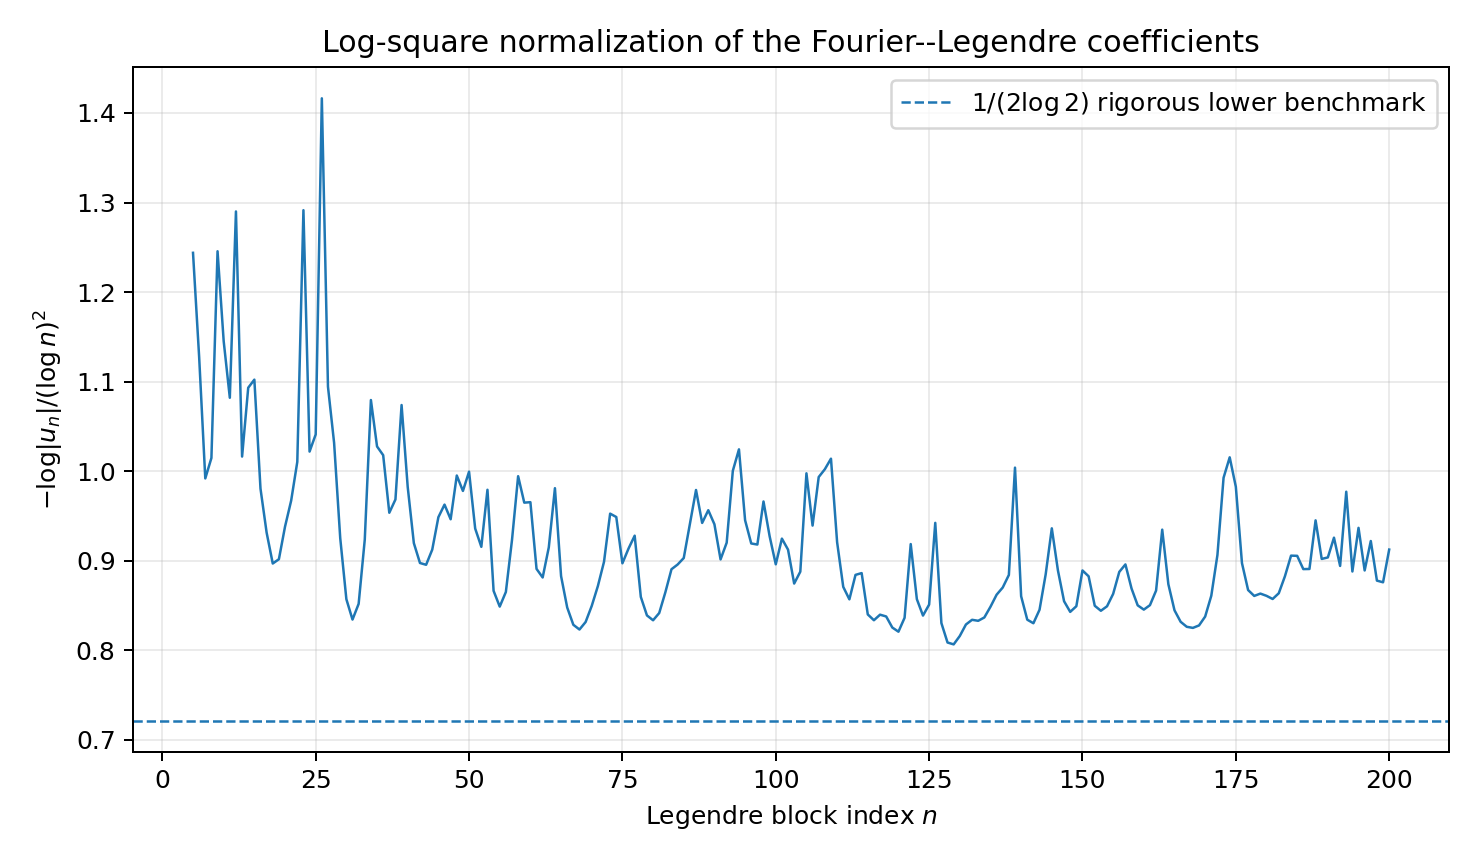
\includegraphics[width=0.94\textwidth]{legendre_decay_ratios.png}
\caption{High-precision values of
$-\log|u_n|/(\log n)^2$ through $n=200$.  The dashed line is the rigorous
benchmark from \cref{thm:un-log-square}.  Oscillation remains substantial,
consistent with a dyadic modulation inherited from the Fourier lobes.}
\label{fig:decay-ratios}
\end{figure}

\section{Two-adic arithmetic of moments and Legendre coefficients}
\label{sec:arithmetic}

\subsection{A proved unit theorem for the moments}

All rational numbers in this subsection are viewed inside $\RationalNumbers_2$.

\begin{theorem}[Every even up-moment is a two-adic unit; new elementary proof]
\label{thm:moment-units}
For every $m\ge0$,
\begin{equation}
 \TwoAdicValuation(\mu_{2m})=0,
 \qquad
 \mu_{2m}\equiv1\pmod2.
 \label{eq:moment-unit}
\end{equation}
\end{theorem}

\begin{proof}
Induct on $m$.  The case $m=0$ is clear.  In
\eqref{eq:moment-recurrence}, every denominator $2r+1$ and the factor
$4^m-1$ are odd.  By induction, each earlier moment is congruent to one modulo
two.  Therefore the right side is congruent to
\[
 \sum_{r=1}^{m}\binom{2m}{2r}
 =2^{2m-1}-1\equiv1\pmod2.
\]
Division by the odd unit $4^m-1$ preserves the congruence.
\end{proof}

\subsection{Experimental congruence patterns}

Exact computation of \eqref{eq:moment-recurrence} through $m=80$ gives the
stronger pattern
\begin{equation}
 \TwoAdicValuation(\mu_{2m}-1)=3+\TwoAdicValuation(m).
 \label{eq:moment-congruence-pattern}
\end{equation}
Independently, the exact moment formula \eqref{eq:un-moments} gives
\begin{equation}
 \TwoAdicValuation(u_n)=-1
 \qquad(0\le n\le80).
 \label{eq:un-v2-data}
\end{equation}
Thus every tested reduced denominator of $u_n$ is twice an odd integer, and
every tested numerator is odd.  In particular, none of the first eighty-one
coefficients vanishes.

\begin{conjecture}[Sharp moment congruence]
\label{conj:moment-congruence}
For every $m\ge1$,
\begin{equation}
 \boxed{\TwoAdicValuation(\mu_{2m}-1)=3+\TwoAdicValuation(m).}
 \label{eq:conj-moment}
\end{equation}
\end{conjecture}

\begin{conjecture}[Half-integrality and nonvanishing of Legendre coefficients]
\label{conj:half-integrality}
For every $n\ge0$,
\begin{equation}
 \boxed{\TwoAdicValuation(u_n)=-1.}
 \label{eq:conj-half-integrality}
\end{equation}
Equivalently, $2u_n$ is a two-adic unit.  In particular $u_n\ne0$ for every
$n$.
\end{conjecture}

A proof of \cref{conj:half-integrality} cannot simply reduce the monomial
formula for $P_{2n}$ modulo two, because its coefficients have large powers of
two in their denominators.  Promising approaches include a two-adic analysis
of the generating function
\[
 \Expectation(1-2tZ+t^2)^{-1/2}
 =\sum_{n\ge0}\Expectation[P_n(Z)]t^n,
\]
or a filtration that combines \cref{conj:moment-congruence} with the exact
Kummer valuations of the Legendre coefficients.

\section{Numerical experiments and independent checks}
\label{sec:numerics}

\subsection{Exact arithmetic layer}

The accompanying program \texttt{experiments.py} uses Python's
\texttt{fractions.Fraction} for:
\begin{itemize}
  \item the moment recurrence \eqref{eq:moment-recurrence};
  \item reciprocal-MGF coefficients from exponential-generating-function
  inversion;
  \item exact monomial coefficients of $P_n$ and $Q_n$;
  \item exact clipped integrals $C_{m,r}(c)$;
  \item exact spectral constants $T_{m\ell r}^{(M)}$ and their partial sums;
  \item two-adic valuations of all reduced rational outputs.
\end{itemize}
No sampled value of $u$ is involved in these calculations.

\subsection{High-precision coefficient layer}

The finite moment expression for $u_n$ has severe alternating cancellation.
The script evaluates moments and coefficient sums with 2300 decimal digits
through $n=200$.  Selected normalized values are
\begin{center}
\begin{tabular}{@{}rrrrrrrrrrr@{}}
\toprule
$n$&20&40&60&80&100&120&140&160&180&200\\
\midrule
$-\log|u_n|/(\log n)^2$
&.9381&.9823&.9654&.8336&.8961&.8208&.8604&.8455&.8609&.9125\\
\bottomrule
\end{tabular}
\end{center}
The rigorous benchmark is
$1/(2\log2)=0.7213475204\ldots$.  The data show no monotone approach and strong
local oscillation.

\subsection{Independent Fourier-product synthesis check}

To check \eqref{eq:legendre-synthesis} without reusing the symbolic proof, the
script evaluates $u$ by inverse FFT of a 42-factor truncation of
\eqref{eq:fourier-product} on a period-eight grid with $2^{18}$ samples.  It
then reconstructs $P_\ell$ from the exact rational coefficients.  The maximum
residuals on 2001 points of $[-1,1]$ are:
\begin{center}
\small
\setlength{\tabcolsep}{4pt}
\begin{tabular}{@{}rrrrrrr@{}}
\toprule
$\ell$&0&1&2&3&4&5\\
\midrule
max residual
&$1.22\!\times10^{-15}$
&$8.88\!\times10^{-16}$
&$3.49\!\times10^{-10}$
&$1.73\!\times10^{-9}$
&$5.19\!\times10^{-9}$
&$1.21\!\times10^{-8}$\\
\bottomrule
\end{tabular}
\end{center}
The growth is expected: exact deconvolution coefficients amplify the small FFT
and interpolation errors increasingly strongly.

\begin{figure}[htbp]
\centering
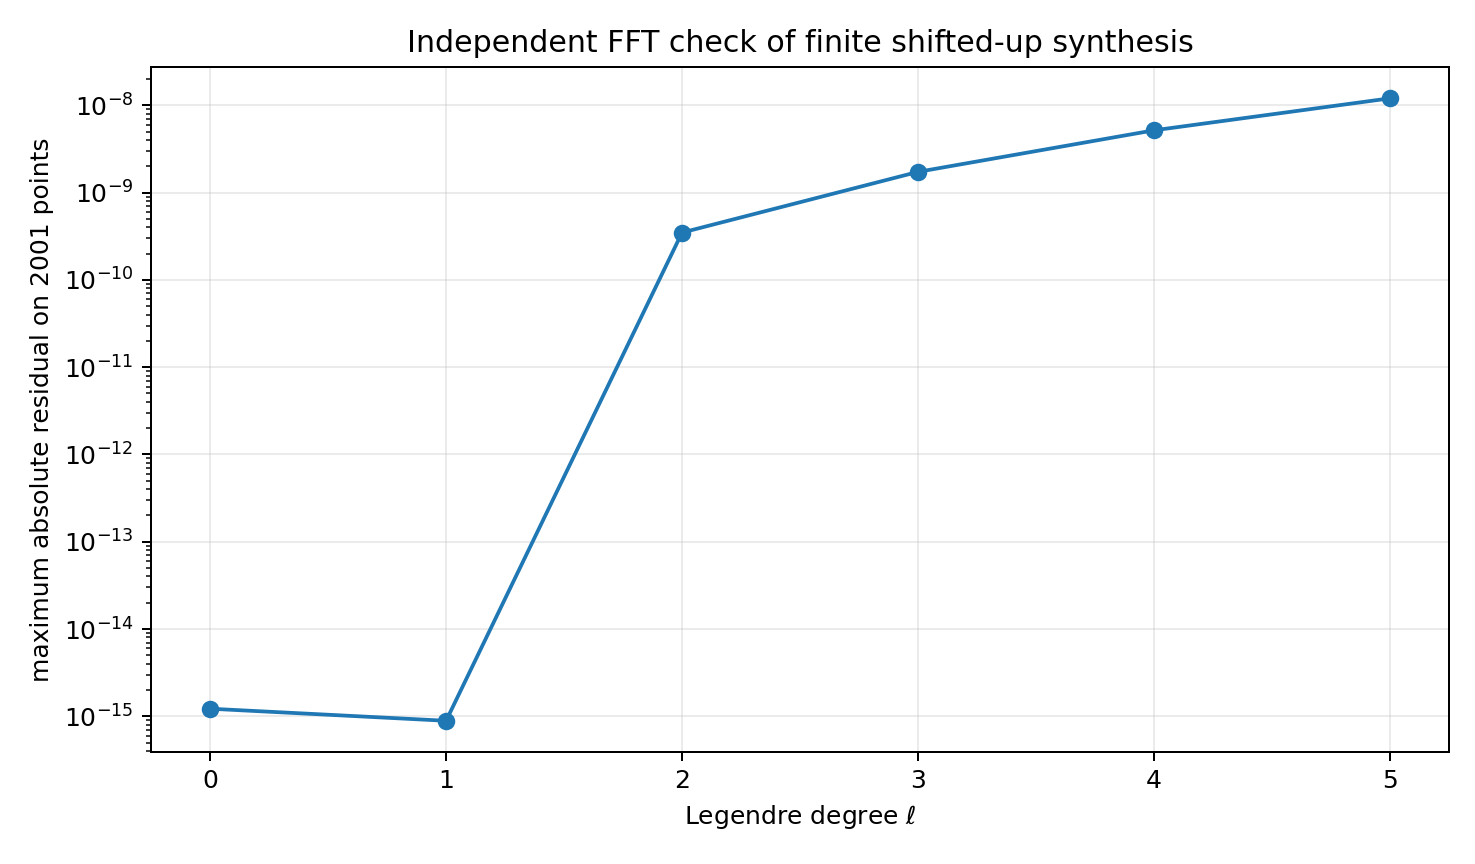
\includegraphics[width=0.92\textwidth]{finite_synthesis_residuals.png}
\caption{Independent numerical residuals of the exact finite synthesis
formula.  The identities themselves are symbolic; the graph measures only
error in the FFT approximation of $u$ and floating evaluation of a
cancellation-prone sum.}
\label{fig:synthesis-residuals}
\end{figure}

\subsection{Reproduction}

From the artifact directory, run
\begin{lstlisting}[style=pythonstyle]
python experiments.py
\end{lstlisting}
The default run regenerates all CSV files, exact TeX snippets, and figures.
Use
\begin{lstlisting}[style=pythonstyle]
python experiments.py --no-plots
\end{lstlisting}
to omit Matplotlib output.  The program requires only NumPy, Matplotlib,
mpmath, and the Python standard library.

\section{Frontier conjectures and research directions}
\label{sec:frontiers}

\subsection{Sharp transfer of the Fourier envelope}

\begin{conjecture}[Sharp log-square constant]
\label{conj:sharp-log-square}
The lower benchmark in \eqref{eq:un-liminf} is sharp:
\begin{equation}
 \boxed{
 \liminf_{n\to\infty}
 \frac{-\log|u_n|}{(\log n)^2}
 =\frac1{2\log2}.}
 \label{eq:conj-sharp-log-square}
\end{equation}
If \cref{conj:half-integrality} holds, no exclusion of zero coefficients is
needed.
\end{conjecture}

The spherical Bessel kernel is concentrated near its turning point
$2\pi|\xi|\asymp2n$, so the conjecture predicts that subsequences of Legendre
coefficients detect near-extremal Fourier lobes rather than suffering an
additional quadratic-log cancellation penalty.

\begin{conjecture}[Dyadic modulation]
\label{conj:dyadic-modulation}
After removing the principal factor
$\exp[-(\log n)^2/(2\log2)]$ and an appropriate power of $n$, the envelope of
$|u_n|$ has a bounded nonconstant modulation depending on the fractional part
of $\log_2 n$.  More precisely, along subsequences
$\{\log_2 n\}\to\theta$, the normalized logarithm should admit a second-order
limit depending periodically on $\theta$.
\end{conjecture}

This is motivated by the exact dyadic shell factorization of $\widehat u$, the
Thue--Morse sign of its Fourier lobes, and the visible oscillations in
\cref{fig:decay-ratios}.  Proving it requires a uniform turning-point
asymptotic for $j_{2n}$ combined with the repository's sharp lobe geometry.

\subsection{Stable spectral biorthogonalization}

The exact matrices $L^{(d)}A^{(d)}=I$ provide a natural starting point for
preconditioning.  The raw synthesis matrix contains factorially growing
columns, but the dual kernel already incorporates the orthogonal projection
that those columns are intended to invert.

\begin{problem}[Optimal diagonal scaling of the spectral pair]
\label{prob:diagonal-scaling}
Find positive row and column weights that minimize
\[
 \Norm{D_1A^{(d)}D_2}_2
 \Norm{D_2^{-1}L^{(d)}D_1^{-1}}_2
\]
subject to exact biorthogonality.  Determine whether the optimal condition
grows subfactorially, and compare literal, oversampled, and compressed atom
dictionaries.
\end{problem}

\begin{problem}[A genuinely stable exact loop]
\label{prob:stable-loop}
Construct a block dictionary or multiscale packet in which the partial
Legendre loop remains exact but the total variation of each block is bounded
by a fixed polynomial in its degree.  The adjacent non-flattening theorem
shows that no naive regrouping of literal atoms can achieve this; the atoms or
analysis functionals must be changed.
\end{problem}

\subsection{Structure of the rational spectral constants}

\begin{question}[Closed forms for $C_{m,r}$ and $T_{m\ell r}^{(M)}$]
\label{question:T-closed-form}
Can the clipped integrals \eqref{eq:Cmr-def} and finite sums
\eqref{eq:T-def} be reduced to terminating hypergeometric or Wigner-symbol
expressions with transparent two-adic valuations?  The unclipped product of
Legendre polynomials is governed by Gaunt coefficients; clipping at an affine
support edge introduces incomplete beta sums.  Their combination with the
Rvachev--Appell samples may conceal a simpler $q$-binomial structure.
\end{question}

\begin{conjecture}[Two-adic boundedness after canonical normalization]
\label{conj:T-v2}
For fixed $m$ and $\ell$, there is an explicit affine function $a(r)$ such
that $2^{a(r)}T_{m\ell r}^{(2^\ell)}$ is a two-adic integer for every $r$, and
the normalized residues form a 2-regular sequence in $r$.
\end{conjecture}

The dyadic clipping endpoints and the $q$-integer annihilator make 2-regularity
a natural possibility.  The exact CSV data are suitable for automated kernel
searches in the sense of Allouche--Shallit \cite{AlloucheShallit2003}.

\subsection{Lambert $W$ and asymptotic thresholds}

The repository uses $W_{-1}$ to invert the small-argument endpoint relation of
the Fabius function and the principal branch $W$ to locate thresholds at which
factorial reciprocal-MGF coefficients dominate prescribed tolerances.  In the
present setting, the asymptotic
$|Q_{2n}(0)|^{1/(2n)}\sim2n/(\pi\EulerE)$ implies that the degree at which the
central atom coefficient reaches size $X$ is governed to first order by
inverting
\[
 2n\log\!\left(\frac{2n}{\pi\EulerE}\right)\asymp\log X,
\]
thus
\begin{equation}
 n\asymp\frac{\log X}{2W(\log X/(\pi\EulerE))}.
 \label{eq:Lambert-threshold}
\end{equation}
A sharper threshold must combine this factorial growth with the log-square and
dyadically modulated decay of $u_n$.

\subsection{Formalization roadmap}

The new results divide cleanly into finite algebra and analytic bridges.
\begin{enumerate}
  \item Define $Q_\ell=\Dscr P_\ell$ in the existing polynomial
  deconvolution API and prove \eqref{eq:Q-jacobi} from the Jacobi derivative
  theorem.
  \item Instantiate the existing synthesis theorem with the Legendre basis and
  package the common-scale matrix $A^{(d)}$.
  \item Define $\Lambda_m$ as a convolution, prove support, smoothness, parity,
  and origin values, then prove $L^{(d)}A^{(d)}=I$ by finite integration.
  \item Formalize clipped intervals and the rational polynomial integral
  $C_{m,r}(c)$; derive the parity theorem and the spectral sum rule.
  \item Reuse the formal Fourier product and spherical-Bessel transform to
  prove \eqref{eq:un-bessel}; then formalize the elementary Bessel and
  log-normal tail estimates in \cref{sec:decay}.
  \item Derive endpoint-flatness sum rules from the already formalized
  $C^\infty$ support properties and Legendre endpoint derivatives.
  \item For the arithmetic conjectures, first formalize
  \cref{thm:moment-units}, then develop two-adic valuations of the exact moment
  and Legendre coefficient recurrences.
\end{enumerate}

\section{Conclusion}
\label{sec:conclusion}

The Legendre specialization of exact up-atom polynomial synthesis is completely
explicit.  Moment deconvolution converts $P_\ell$ into a rational
Bell--Bernoulli/Jacobi polynomial $Q_\ell$; dyadic samples of $Q_\ell$ are the
coefficients of a finite literal-shift representation on $[-1,1]$.  The
repository's minimal local dictionary compresses the same polynomial to
$\ell+2$ dilated atoms.

Substitution into the canonical Fourier--Legendre expansion closes the loop
exactly.  The correct object is an absolutely convergent series of finite
cancellation blocks.  The factorial growth of deconvolution and the adjacent
non-flattening theorem rule out a naive unconditional atom series.

The dual kernel $\Lambda_m$ reveals more than the requested composition.  It
turns the shifted atom system into an exact spectral analysis/synthesis pair,
with $L^{(d)}A^{(d)}=I$.  Expanding shifted atoms locally produces infinite
rational identities for the canonical coefficients, while endpoint flatness
produces an independent hierarchy of weighted cancellation laws.  The
spherical-Bessel representation connects Legendre coefficients directly to
the dyadic sinc-product envelope and yields a quantitative log-square decay
theorem.

The remaining frontier is not existence but structure: sharp oscillatory
asymptotics, stable preconditioning, two-adic integrality, and closed forms for
the rational spectral constants.  These questions now have exact finite
objects, reproducible data, and a clear route toward Lean formalization.

\appendix

\section{Exact formulae used by the experiment program}
\label{app:formulae}

For reference, the reciprocal EGF recurrence is
\begin{equation}
 \gamma_{2m}=-\sum_{r=1}^{m}\binom{2m}{2r}
 \mu_{2r}\gamma_{2m-2r}.
 \label{eq:gamma-recurrence}
\end{equation}
If
\[
 P_\ell(x)=\sum_{j=0}^{\ell}p_{\ell,j}x^j,
\]
then the exact monomial form of $Q_\ell$ is
\begin{equation}
 Q_\ell(x)=\sum_{j=0}^{\ell}p_{\ell,j}
 \sum_{r=0}^{\Floor{j/2}}
 \binom{j}{2r}\gamma_{2r}x^{j-2r}.
 \label{eq:Q-monomial}
\end{equation}
For rational $c$, the code evaluates
\begin{equation}
 C_{m,r}(c)=\frac{2m+1}{2}
 \int_{\max(-1,c-1)}^{\min(1,c+1)}
 P_m(x)P_{2r}(x-c)\Differential x
 \label{eq:C-code}
\end{equation}
by exact polynomial multiplication and antiderivatives.

\section{Artifact inventory}
\label{app:inventory}

The accompanying archive contains:
\begin{itemize}
  \item \texttt{legendre\_rvachev\_closed\_loop.tex} and the compiled PDF;
  \item \texttt{experiments.py}, with detailed comments and command-line
  options;
  \item \texttt{README.txt} and \texttt{MANIFEST.txt};
  \item exact CSV data for moments, reciprocal coefficients, Legendre
  coefficients, spectral sum rules, and synthesis checks;
  \item a multiprecision CSV file for the coefficient-decay experiment;
  \item the generated TeX snippets and PNG figures used in the report.
\end{itemize}

\begin{thebibliography}{99}

\bibitem{Fabius1966}
J.~Fabius,
\newblock A probabilistic example of a nowhere analytic $C^\infty$-function,
\newblock \emph{Zeitschrift f\"ur Wahrscheinlichkeitstheorie und Verwandte
Gebiete} \textbf{5} (1966), 173--174.

\bibitem{Rvachev1971}
V.~L.~Rvachev and V.~A.~Rvachev,
\newblock A certain finite function,
\newblock \emph{Dopovidi Akademii Nauk Ukrains'koi RSR, Series A} (1971),
705--707, 764.

\bibitem{Rvachev1972}
V.~L.~Rvachev and V.~A.~Rvachev,
\newblock On the representation of polynomials by functions with compact
support,
\newblock \emph{Mathematical Physics}, No.~11, Naukova Dumka, Kiev, 1972,
126--129.

\bibitem{Rvachev1990}
V.~A.~Rvachev,
\newblock Compactly supported solutions of functional-differential equations
and their applications,
\newblock \emph{Russian Mathematical Surveys} \textbf{45} (1990), no.~1,
87--120.

\bibitem{Arias1982}
J.~Arias de Reyna,
\newblock Definici\'on y estudio de una funci\'on indefinidamente diferenciable
de soporte compacto,
\newblock \emph{Rev. Real Acad. Ciencias Madrid} \textbf{76} (1982), 21--38;
English translation arXiv:1702.05442.

\bibitem{Arias2018}
J.~Arias de Reyna,
\newblock Arithmetic of the Fabius function,
\newblock \emph{INTEGERS} \textbf{18} (2018), Article A51.

\bibitem{StrangFix1973}
G.~Strang and G.~Fix,
\newblock A Fourier analysis of the finite element variational method,
\newblock in \emph{Constructive Aspects of Functional Analysis}, C.I.M.E.,
1973, pp.~793--840.

\bibitem{Szego1975}
G.~Szeg\H{o},
\newblock \emph{Orthogonal Polynomials}, 4th ed.,
\newblock American Mathematical Society Colloquium Publications, Vol.~23,
1975.

\bibitem{Watson1944}
G.~N.~Watson,
\newblock \emph{A Treatise on the Theory of Bessel Functions}, 2nd ed.,
\newblock Cambridge University Press, 1944.

\bibitem{Roman1984}
S.~Roman,
\newblock \emph{The Umbral Calculus},
\newblock Academic Press, 1984.

\bibitem{Comtet1974}
L.~Comtet,
\newblock \emph{Advanced Combinatorics},
\newblock Reidel, 1974.

\bibitem{AlloucheShallit2003}
J.-P.~Allouche and J.~Shallit,
\newblock \emph{Automatic Sequences: Theory, Applications, Generalizations},
\newblock Cambridge University Press, 2003.

\bibitem{ProveItPrimary}
V.~Reshetnikov,
\newblock \emph{The Fabius Function and Rvachev's Up-Function},
\newblock canonical primary exposition in the \texttt{ProveIt} repository,
\repo, snapshot 29 August 2026.

\bibitem{ProveItPoly}
V.~Reshetnikov,
\newblock \emph{Exact Polynomial Synthesis from Rvachev Up-Atoms},
\newblock consolidated frontier volume in the \texttt{ProveIt} repository,
\nolinkurl{semi-formalized-research-frontiers/drafts/representations/Up_Polynomial_Synthesis/},
28 August 2026.

\bibitem{ProveItLagrange}
V.~Reshetnikov,
\newblock \emph{Closing the Lagrange--Legendre--Rvachev Loop},
\newblock adjacent frontier report in the \texttt{ProveIt} repository,
\nolinkurl{semi-formalized-research-frontiers/drafts/representations/lagrange_rvachev_loop_report_v3/},
29 August 2026.

\end{thebibliography}

\end{document}
